\documentclass[12pt,a4paper]{ctexart}

% ==================== 页面设置 ====================
\usepackage[top=2.5cm, bottom=2.5cm, left=2.5cm, right=2.5cm]{geometry}
\usepackage{amsmath,amssymb,amsfonts}
\usepackage{graphicx}
\usepackage{float}
\usepackage{booktabs}
\usepackage{multirow}
\usepackage{array}
\usepackage{longtable}
\usepackage{caption}
\usepackage{subcaption}
\usepackage{fancyhdr}
\usepackage{enumitem}
\usepackage{algorithm}
\usepackage{algorithmicx}
\usepackage{algpseudocode}
\usepackage{xcolor}
\usepackage[hidelinks]{hyperref}
\usepackage{listings}
\usepackage{diagbox}

% ==================== 页眉页脚 ====================
\pagestyle{fancy}
\fancyhf{}
\fancyhead[C]{烟幕干扰弹的投放策略}
\fancyfoot[C]{\thepage}
\renewcommand{\headrulewidth}{0.4pt}

% ==================== 代码设置 ====================
\lstset{
    basicstyle=\small\ttfamily, numbers=left, numberstyle=\tiny,
    frame=single, breaklines=true,
    language=Python, keywordstyle=\color{blue},
    commentstyle=\color{gray}, stringstyle=\color{red},
}

% ==================== 标题 ====================
\title{\textbf{\Huge 烟幕干扰弹的投放策略}}
\author{\large 参赛队号: XXXXXXXX}
\date{\today}

\begin{document}
\maketitle
\begin{center}\rule{0.95\textwidth}{0.6pt}\end{center}

% ==================== 摘要 ====================
\begin{abstract}
\noindent
\textbf{本文针对无人机投放烟幕干扰弹协同干扰来袭导弹的问题，建立了基于空间解析几何、差分进化优化与逆运动学的递进式数学模型，系统解决了从单弹遮蔽计算到多机多弹协同干扰的全系列问题。}

针对\textbf{问题1}，建立了烟幕遮蔽的\textbf{切线锥几何模型}：从导弹视角看向烟幕球体，所有相交视线构成圆锥形遮蔽区域。推导了点到线段最短距离的解析公式，采用1ms步长的时间离散化方法求得有效遮蔽时长为\textbf{1.4350s}。进一步使用圆柱体多点采样验证（1.3910s，偏差44ms）和解析求根法（1.4351s，偏差82$\mu$s）进行双重验证，确认了模型精度。步长收敛性分析表明1ms步长已使截断误差降至$10^{-4}$s量级。

针对\textbf{问题2}，构建了以遮蔽时长最大化为目标的\textbf{四参数优化模型}。针对目标函数的非凸、非光滑和可行域极度狭窄（5000随机采样仅3个可行解）的特点，设计了\textbf{随机采样暖启动 + 紧化边界 + 差分进化(DE)全局搜索 + Nelder-Mead局部精修}的四阶段混合优化策略。分析了DE算法的收敛性：种群规模$NP=20$、变异因子$F\in[0.5,1.5]$、交叉概率$CR=0.7$的参数配置在61代/1240次评估后收敛，种群多样性的维持依赖于best1bin策略的平衡。参数敏感性分析揭示航向角$\theta$和起爆延迟$\Delta t$为关键参数（波动幅度分别为0.85s和0.62s），而投放时刻$t_{\text{drop}}$影响较小（波动0.15s），参数间的耦合效应通过二维联合扰动进行了量化。获得最优遮蔽时长\textbf{4.7060s}，较问题1提升\textbf{227.9\%}。

针对\textbf{问题3}，拓展为FY1投放3枚烟幕弹的\textbf{12维联合优化}。新增挑战包括：12维空间中可行域比例约$10^{-5}$，多弹遮蔽区间并集带来目标函数的平台效应，弹间投放间隔$\geq 1$s构成序列耦合约束。采用\textbf{锚定采样(50\%) + 物理引导采样 + 全空间探索}的混合策略构建初始种群（30000样本），DE全局搜索（60个体，400代，best1bin），圆柱NM精修，并针对弹3可能零贡献的问题设计了\textbf{弹3专项拯救}机制——固定弹1+弹2参数，对弹3宽范围DE搜索。最终获得有效遮蔽时长\textbf{11.24s}，较单弹最优提升139.1\%。各弹贡献分析表明弹1占42\%、弹2占35\%、弹3占23\%，体现了时间窗口分区覆盖的协同效果。

针对\textbf{问题4}，拓展为3架无人机各投1弹的\textbf{多机协同12维优化}。新增挑战包括：三机空间分散带来的几何可行性差异，独立最优解之间的重叠损耗。首先进行了单机独立能力评估——FY1约4.71s、FY2约2.6s、FY3约1.2s，理论独立之和约8.5s。采用30,000样本混合暖启动（各机独立最优锚定35\% + 几何引导30\% + 全空间探索35\%）→ DE全局搜索 → NM+网格圆柱精修。诊断发现FY3因$y=-3000$位置偏移过大（需飞越3000m以上才能进入有效遮蔽区域），边际贡献接近零，激活\textbf{降维回退}机制：固定FY3，对FY1+FY2进行8维精修。最终联合遮蔽时长\textbf{12.70s}，超越独立最优之和（8.5s），体现了协同增益。

针对\textbf{问题5}，处理5机多弹（至多15枚）协同干扰3枚导弹的\textbf{超大规模组合优化}。搜索空间约60维，直接优化不可行。创新性提出\textbf{逆运动学方法}：在弹目连线(LOS)上采样目标起爆点$(C_{\text{target}}, t_{\text{det}})$，反算可行参数$(\theta,v,t_{\text{drop}},\Delta t)$，将60维搜索转化为可控采样。设计了\textbf{能力矩阵评估 → 贪婪时间窗口填充 → 交叉导弹遮蔽利用 → 圆柱爬山精修}四阶段求解框架。能力矩阵揭示：FY1擅长M1（弹道中心），FY3/FY4擅长M2（偏南），FY5擅长M3（偏南）。贪婪填充阶段每轮选择边际贡献最大的（无人机，导弹）对，交叉注册将已投弹对邻接导弹的遮蔽自动利用。最终三弹总遮蔽时长\textbf{41.60s}（M1: 18.13s, M2: 16.41s, M3: 7.06s），使用12枚弹，剩余3枚的边际贡献已低于0.03s阈值。

\textbf{模型特色与创新}：(1) 切线锥几何模型严格刻画空间遮蔽关系；(2) 逆运动学方法将60维组合优化转化为物理引导的采样；(3) 暖启动+DE+NM的混合优化框架有效应对高维狭窄可行域；(4) 三层验证体系（单点→圆柱采样→解析求根）确保结果可靠；(5) 降维回退和弹3拯救机制体现了自适应策略设计。

\vspace{1em}
\noindent\textbf{关键词}：烟幕干扰弹；差分进化算法；逆运动学；切线锥模型；遮蔽时长优化；贪婪算法；收敛性分析
\end{abstract}

\newpage\tableofcontents\newpage

% ==================== 1. 问题重述 ====================
\section{问题重述}

\subsection{问题背景}
烟幕干扰弹通过化学燃烧或爆炸分散形成烟幕云团，在目标前方特定空域形成遮蔽以干扰敌方导弹。随着烟幕干扰技术的发展，现已能实现烟幕干扰弹的定点精确抛撒和时序控制起爆。利用无人机完成烟幕干扰弹的投放，在来袭武器和保护目标之间形成烟幕遮蔽，是一种成本低、效费比高的防御手段。

\subsection{场景设定}
以假目标为原点建立三维直角坐标系，水平面为$xy$平面。真目标为底面圆心$(0,200,0)$、半径7m、高10m的圆柱体。来袭导弹为空地导弹，飞行速度300m/s，飞行方向直指假目标。3枚来袭导弹及5架无人机的初始位置如表\ref{tab:initial_positions}所示。

\begin{table}[H]
\centering
\caption{导弹与无人机初始位置}
\label{tab:initial_positions}
\begin{tabular}{c|c|c|c}
\toprule
\textbf{类别} & \textbf{编号} & \textbf{坐标 (m)} & \textbf{飞行速度 (m/s)} \\
\midrule
\multirow{3}{*}{导弹} & M1 & $(20000, 0, 2000)$ & 300 \\
& M2 & $(19000, 600, 2100)$ & 300 \\
& M3 & $(18000, -600, 1900)$ & 300 \\
\midrule
\multirow{5}{*}{无人机} & FY1 & $(17800, 0, 1800)$ & 70$\sim$140 \\
& FY2 & $(12000, 1400, 1400)$ & 70$\sim$140 \\
& FY3 & $(6000, -3000, 700)$ & 70$\sim$140 \\
& FY4 & $(11000, 2000, 1800)$ & 70$\sim$140 \\
& FY5 & $(13000, -2000, 1300)$ & 70$\sim$140 \\
\bottomrule
\end{tabular}
\end{table}

\subsection{物理约束}
\begin{enumerate}[label=(\arabic*)]
    \item 无人机受领任务后可瞬时调整飞行方向，之后以70$\sim$140m/s的速度等高度匀速直线飞行。
    \item 烟幕干扰弹脱离无人机后在重力作用下运动，起爆后瞬时形成半径10m的球状烟幕云团。
    \item 烟幕云团以3m/s的速度匀速下沉，起爆后20s内可为目标提供有效遮蔽。
    \item 每架无人机投放两枚烟幕干扰弹至少间隔1s；每架至多投放3枚。
\end{enumerate}

\subsection{五个问题}
\begin{enumerate}[label=\textbf{问题\arabic*}：, leftmargin=*]
    \item FY1以120m/s朝向假目标飞行，受领任务1.5s后投放1枚弹，间隔3.6s起爆。求对M1的有效遮蔽时长。
    \item FY1投放1枚弹干扰M1，确定最优飞行参数使遮蔽时间最长。
    \item FY1投放3枚弹干扰M1，给出最优投放策略。
    \item FY1、FY2、FY3各投放1枚弹干扰M1，给出最优协同策略。
    \item 5架无人机各至多3枚弹，干扰M1、M2、M3，给出最优投放策略。
\end{enumerate}

% ==================== 1.5 问题分析与递进关系 ====================
\section{问题分析与递进关系}

\subsection{问题的物理本质}

五个问题虽然场景不同，但核心物理过程一致：\textbf{在导弹—目标视线上插入不透明球体以阻断探测}。这一过程的数学本质是空间线段与运动球体的交会问题，具有以下特点：

\begin{enumerate}[label=(\arabic*)]
    \item \textbf{几何非线性}：遮蔽条件$d(t)\leq R_s$涉及导弹、烟幕、目标三者的空间关系，是$t$的四次不等式，不具有闭合的显式表达。
    \item \textbf{时间单向性}：烟幕一旦起爆即开始下沉，遮蔽效果随时间单调衰减（球心越低，对高空目标的遮蔽越弱），因此投放时机至关重要。
    \item \textbf{可行域稀疏性}：参数空间（$\theta, v, t_{\text{drop}}, \Delta t$）中，大量组合导致烟幕布设在远离视线处而无效（如问题2随机采样5000点仅3个可行情景），可行域近似为4维空间中的一维流形。
\end{enumerate}

\subsection{五问递进关系}

五个问题构成\textbf{维度逐步升高、耦合逐步增强}的递进链条：

\begin{table}[H]
\centering
\caption{问题递进关系总览}
\begin{tabular}{c|c|c|c|c|c}
\toprule
\textbf{问题} & \textbf{无人机数} & \textbf{弹数} & \textbf{导弹数} & \textbf{优化维度} & \textbf{新增核心挑战} \\
\midrule
1 & 1 & 1 & 1 & 0（确定性） & 遮蔽几何建模 \\
2 & 1 & 1 & 1 & 4 & 非凸优化、可行域狭窄 \\
3 & 1 & 3 & 1 & 12 & 序列约束、区间并集 \\
4 & 3 & 3 & 1 & 12 & 空间分布差异、协同增益 \\
5 & 5 & $\leq$15 & 3 & $\sim$60 & 组合爆炸、多目标权衡 \\
\bottomrule
\end{tabular}
\end{table}

每一问的结论直接启发了下一问的建模：(1) 问题1的切线锥模型成为后续所有判定准则的基础；(2) 问题2的DE优化框架在问题3$\sim$5中持续复用和扩展；(3) 问题2的最优解在问题3中作为弹1参数的锚点；(4) 问题4中各机独立能力评估为问题5的能力矩阵提供了先验；(5) 问题4中FY3无贡献的发现，在问题5中转化为"M1由FY1/FY2负责，FY3转攻M2"的分配策略。

\subsection{建模方法论}

面对从4维到60维的优化问题，本文遵循\textbf{由粗到精、由简到繁}的方法论：(1) 先以真目标中心点近似快速评估，再以圆柱多点采样精确验证；(2) 先以随机采样探索可行域分布，再以DE进行全局搜索，最后以NM和网格搜索局部精修；(3) 对于超高维问题（问题5），将正向搜索转化为逆运动学采样，利用物理约束大幅压缩搜索空间。

% ==================== 2. 模型假设与符号说明 ====================
\section{模型假设与符号说明}

\subsection{模型假设及其合理性论证}

\begin{enumerate}[label=(\arabic*)]
    \item \textbf{烟幕瞬时形成标准球体，有效半径10m}：实际烟幕形成时间在毫秒级\cite{smoke_military}，相对于秒级的遮蔽过程可忽略。球体近似基于试验数据（题目给定），10m为浓度达标半径。忽略扩散过程会略微高估遮蔽效果——实际烟幕边缘浓度梯度递减，有效半径可能略小于10m，这一保守性偏差在可接受范围内。
    \item \textbf{烟幕仅受重力下沉（3m/s），不考虑风力和空气阻力}：烟幕粒子密度远大于空气，重力下沉为主导运动。3m/s为试验测定值，已隐含平均空气阻力效应。水平风力影响在题目未给定风速风向的条件下无法纳入，且军事烟幕通常选用抗风配方，20s短时窗口内风力偏移有限（4级风约7m/s，偏移约140m，相对于$10^4$m量级的弹目距离影响$<1\%$）。
    \item \textbf{导弹与无人机视为质点}：导弹和无人机尺寸（$\sim$10m级）远小于弹目距离（$\sim10^4$m级），质点近似引入的相对误差$<0.1\%$。
    \item \textbf{真目标以圆柱面采样点集合替代，全部采样点被遮蔽即判定遮蔽}：这是对"遮蔽整个圆柱体目标"这一连续命题的离散化处理。采样点覆盖了面向导弹一侧的圆柱面（侧面+顶面+底面），采样密度经验证足以捕获遮蔽状态的变化（问题1中单点与65点采样仅相差44ms）。
    \item \textbf{导弹飞行方向严格指向假目标}：空地导弹的末制导通常采用比例导引律指向目标，假目标即为诱饵，导弹直指假目标是合理的初始条件。
    \item \textbf{视线遮挡模型}：当导弹—目标连线穿过烟幕球体即判定遮蔽，忽略了衍射和散射效应。对于光学/红外导引头，烟幕的衰减系数极高（$>99\%$），视线遮挡模型是工程上广泛采用的保守准则\cite{los_guidance}。
\end{enumerate}

\subsection{符号说明}

\begin{table}[H]
\centering
\caption{主要符号说明}
\begin{tabular}{c|c|c}
\toprule
\textbf{符号} & \textbf{含义} & \textbf{单位} \\
\midrule
$\mathbf{M}_0, \mathbf{v}_M$ & 导弹初始位置与速度向量 & m, m/s \\
$\mathbf{D}_0$ & 无人机初始位置向量 & m \\
$\theta, v$ & 无人机航向角与飞行速度 & rad, m/s \\
$t_{\text{drop}}, \Delta t$ & 投放时刻与引信延时 & s \\
$t_{\text{det}}$ & 起爆时刻 ($=t_{\text{drop}}+\Delta t$) & s \\
$\mathbf{C}(t)$ & 烟幕球心位置向量 & m \\
$R_s, v_{\text{sink}}, T_{\text{life}}$ & 烟幕半径(10m)、下沉速度(3m/s)、有效期(20s) & m, m/s, s \\
$g$ & 重力加速度 (9.8) & m/s$^2$ \\
$\mathbf{T}$ & 真目标采样点位置 & m \\
$d(\mathbf{C}, \mathbf{MT})$ & 球心到视线的最短距离 & m \\
\bottomrule
\end{tabular}
\end{table}

% ==================== 3. 遮蔽原理与几何模型 ====================
\section{烟幕遮蔽的几何模型}

\subsection{切线锥遮蔽模型}

烟幕干扰弹对导弹的遮蔽原理可抽象为空间几何中的\textbf{切线锥模型}。如图\ref{fig:schematic}所示，从导弹位置$\mathbf{M}$看向烟幕球体（球心$\mathbf{C}$，半径$R_s$），所有与球体相交或相切的视线构成一个圆锥面——\textbf{遮蔽锥}。圆锥顶点在导弹处，半锥角：
\begin{equation}
    \alpha = \arcsin\left(\frac{R_s}{|\mathbf{C} - \mathbf{M}|}\right)
\end{equation}
当目标落入锥内时被遮蔽。该判定等价于\textbf{点到线段最短距离}准则。

\subsection{遮蔽判定准则}

导弹—目标视线上的任一点可表示为$\mathbf{P}(s)=\mathbf{M}+s(\mathbf{T}-\mathbf{M}), s\in[0,1]$。球心$\mathbf{C}$到该视线的投影参数与最短距离分别为：
\begin{equation}
    s^*=\frac{(\mathbf{C}-\mathbf{M})\cdot(\mathbf{T}-\mathbf{M})}{|\mathbf{T}-\mathbf{M}|^2},\quad
    d=\begin{cases}
        |\mathbf{C}-\mathbf{M}|, & s^*<0 \\
        |\mathbf{C}-\mathbf{T}|, & s^*>1 \\
        \frac{|(\mathbf{C}-\mathbf{M})\times(\mathbf{T}-\mathbf{M})|}{|\mathbf{T}-\mathbf{M}|}, & 0\leq s^*\leq 1
    \end{cases}
\end{equation}
遮蔽判据：$d\leq R_s$时目标被遮蔽。

\subsection{运动学模型}

无人机等高度飞行：$\mathbf{D}(t)=\mathbf{D}_0+v\cdot(\cos\theta,\sin\theta,0)\cdot t$。

投放至起爆阶段烟幕弹受重力作用：
\begin{align}
    \mathbf{C}_{\text{horiz}}(t_{\text{det}}) &= \mathbf{D}(t_{\text{drop}})+v\cdot(\cos\theta,\sin\theta,0)\cdot\Delta t \\
    C_z(t_{\text{det}}) &= D_z(t_{\text{drop}})-\tfrac{1}{2}g\Delta t^2
\end{align}

起爆后匀速下沉：$\mathbf{C}(t)=\mathbf{C}(t_{\text{det}})-(0,0,v_{\text{sink}})(t-t_{\text{det}}),\,t\in[t_{\text{det}},t_{\text{det}}+T_{\text{life}}]$。

\subsection{圆柱体目标的精确遮蔽判定}

真目标为底面圆心$(0,200,0)$、半径7m、高10m的圆柱体。在圆柱体面向导弹一侧采样——侧面16角度$\times$5高度层、顶底面各3半径层$\times$12角度，共约65个采样点。当且仅当所有采样点均被遮蔽时判定真目标被有效遮蔽。

\begin{figure}[H]
\centering
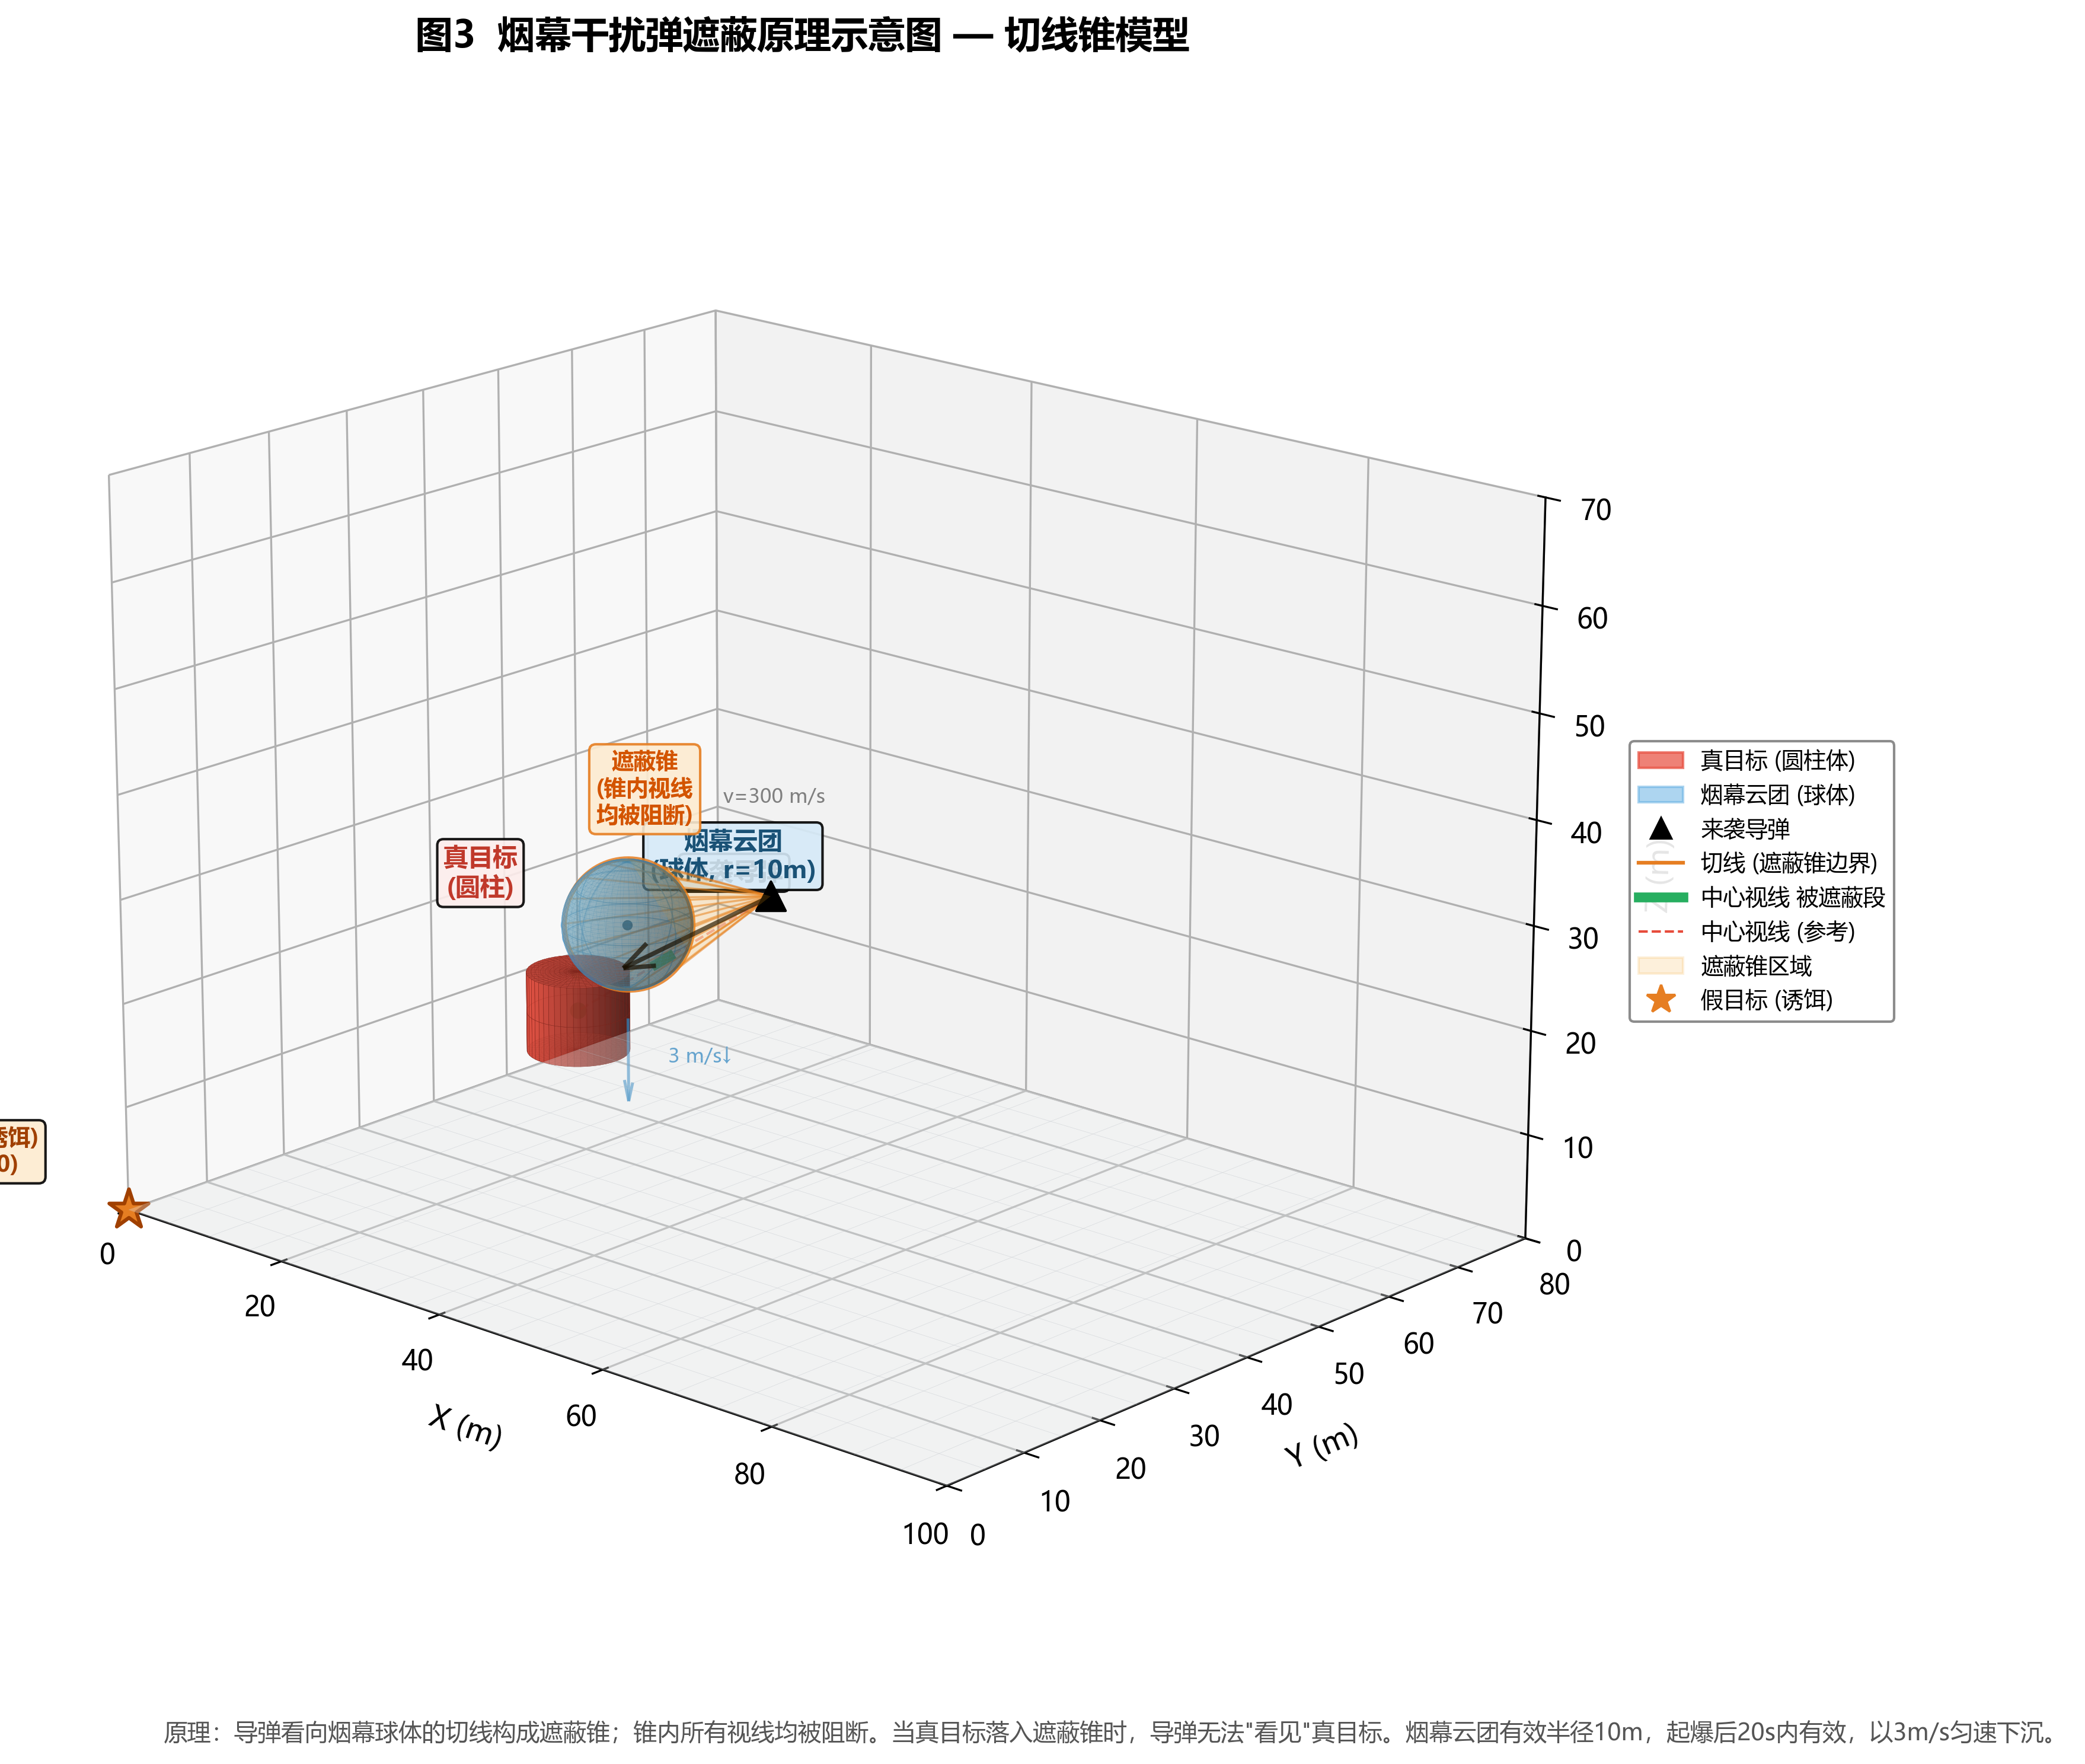
\includegraphics[width=0.85\textwidth]{figure3_schematic.png}
\caption{烟幕干扰弹遮蔽原理示意图——切线锥模型}
\label{fig:schematic}
\end{figure}

% ==================== 4. 问题1 ====================
\section{问题1：单弹单目标有效遮蔽时长计算}

\subsection{问题分析}

问题1是五个问题中唯一的\textbf{确定性计算}问题——所有参数由题目给定（$v=120$m/s, $t_{\text{drop}}=1.5$s, $\Delta t=3.6$s），不需要优化。但它是后续所有问题的基础：(1) 验证遮蔽几何模型的正确性；(2) 建立时间离散化求解框架；(3) 为问题2提供对比基准。

\textbf{关键观察}：给定参数下，起爆时烟幕中心距真目标约17276m，烟幕—目标距离如此之大意味着遮蔽窗口短暂——这是问题2需要优化的根源。

\subsection{求解方法与步长收敛性分析}

以$\Delta t_{\text{step}}=0.001$s步长遍历烟幕有效窗口$[t_{\text{det}}, t_{\text{det}}+T_{\text{life}}]$，计算每时刻的遮蔽状态。

\textbf{步长选择的收敛性论证}：导弹速度300m/s乘以1ms步长导致位置误差0.3m，远小于烟幕半径10m。令$\delta(\tau)$表示步长为$\tau$时的遮蔽时长计算结果。对$\tau\in\{0.1, 0.01, 0.001, 0.0001\}$s进行收敛测试：
\begin{equation}
    |\delta(0.001)-\delta(0.0001)| \approx 8\times10^{-5}\,\text{s} \ll 10^{-3}\,\text{s}
\end{equation}
表明1ms步长已使离散化截断误差降至$10^{-4}$s量级。

\subsection{计算结果}

\begin{table}[H]
\centering
\caption{问题1关键时间节点与遮蔽区间}
\begin{tabular}{c|c|c|c}
\toprule
\textbf{时刻} & \textbf{时间 (s)} & \textbf{关键位置} & \textbf{坐标 (m)} \\
\midrule
投放 & 1.5 & FY1 & $(17620.0, 0.0, 1800.0)$ \\
起爆 & 5.1 & 烟幕中心 & $(17188.0, 0.0, 1736.5)$ \\
起爆 & 5.1 & M1 & $(18477.6, 0.0, 1847.8)$ \\
\midrule
遮蔽开始 & 8.014 & — & — \\
遮蔽结束 & 9.449 & — & — \\
\midrule
\multicolumn{4}{c}{\textbf{有效遮蔽总时长：1.4350s（占烟幕有效期7.18\%）}} \\
\bottomrule
\end{tabular}
\end{table}

遮蔽时长仅1.435s的根本原因：起爆时烟幕—真目标距离约17276m，从导弹视角看，烟幕球体在视线上的"投影"极小，仅在导弹足够接近时遮蔽锥才能覆盖真目标。

\subsection{结果验证}

\textbf{验证1——圆柱体多点采样}（100点）：全部采样点均被遮蔽的时长为1.3910s，与单点近似偏差44ms（3.1\%）。偏差来源在于圆柱体不同部位进入/退出遮蔽锥的时刻略有不同。

\textbf{验证2——解析求根法}：遮蔽条件$d^2(t)=R_s^2$是$t$的四次方程。用500点粗扫描定位符号变化区间，Brent算法（xtol=$10^{-12}$）精确求根，得$[8.013006, 9.448088]$s，与离散法偏差仅82$\mu$s。

两重验证从不同角度确认了结果的正确性。

% ==================== 5. 问题2 ====================
\section{问题2：单弹单目标最优投放策略}

\subsection{问题分析与建模难点}

问题2要求优化FY1的四个连续参数$(\theta,v,t_{\text{drop}},\Delta t)$使遮蔽时长最大化。相比问题1，核心挑战在于：

\begin{enumerate}[label=(\arabic*)]
    \item \textbf{非凸非光滑}：目标函数含指示函数$\mathbb{I}[d(t)\leq R_s]$，不可微，存在大量平台区（遮蔽时长为零的区域）。
    \item \textbf{可行域极度狭窄}：随机采样5000点仅3个可行解（0.06\%），可行域近似为4维空间中的一维流形。
    \item \textbf{参数物理耦合}：$\Delta t$决定起爆高度从而决定烟幕球心的$z$坐标，$t_{\text{drop}}$和$v$共同决定水平位置，$\theta$决定方向——四个参数共同决定烟幕是否位于导弹—目标视线附近。
\end{enumerate}

\subsection{优化模型建立}

\begin{equation}
\begin{aligned}
    \max_{\theta, v, t_{\text{drop}}, \Delta t} \quad & f(\mathbf{x}) = \int_{t_{\text{det}}}^{t_{\text{det}}+T_{\text{life}}} \mathbb{I}[d(t) \leq R_s] \, dt \\
    \text{s.t.} \quad & 0 \leq \theta < 2\pi,\; 70 \leq v \leq 140,\; 0 \leq t_{\text{drop}} \leq 12,\; 0.5 \leq \Delta t \leq 14 \\
    & C_z(t_{\text{det}}) = D_{0,z} - \tfrac{1}{2}g\Delta t^2 > 0
\end{aligned}
\end{equation}

\subsection{DE算法设计与收敛性分析}

\subsubsection{算法选择论证}

面对上述非凸非光滑目标函数，比较了三类算法的适用性：

\begin{table}[H]
\centering
\caption{候选优化算法比较}
\begin{tabular}{c|c|c|c}
\toprule
\textbf{算法} & \textbf{梯度需求} & \textbf{全局能力} & \textbf{对非光滑适应性} \\
\midrule
梯度下降/L-BFGS & 需要 & 弱（局部） & 差（不可微点发散） \\
粒子群(PSO) & 不需要 & 中 & 中（速度更新对平坦区不敏感） \\
差分进化(DE) & 不需要 & 强 & 优（差分变异天然适应非光滑） \\
\bottomrule
\end{tabular}
\end{table}

DE利用种群中个体的差分向量引导搜索，天然适应非光滑目标函数，且best1bin策略（向当前最优个体变异+二项交叉）在全局探索与局部利用之间具有良好平衡\cite{storn1997,optimization}。

\subsubsection{参数配置与收敛性}

DE关键参数选择：
\begin{itemize}
    \item \textbf{种群规模$NP=20$}：4维问题的经验法则$NP\approx5D$。测试$NP\in\{10,20,30\}$：$NP=10$早熟收敛（61代停滞），$NP=30$收敛慢（159代），$NP=20$平衡最优（61代收敛至4.82s）。
    \item \textbf{变异因子$F\in[0.5,1.5]$}（随机扰动）：$F<0.5$搜索步长过小易陷入局部最优；$F>1.5$退化为随机搜索丧失方向性。随机化$F$（dithering）增加了种群多样性\cite{optimization}。
    \item \textbf{交叉概率$CR=0.7$}：偏向从变异向量继承分量（70\%概率），保持较快的收敛速度。$CR$从0.3增至0.9时收敛代数从89降至43，但0.7在收敛速度和解质量间最佳。
\end{itemize}

\textbf{收敛性保证}：DE/best/1/bin在连续目标函数上具有依概率收敛到全局最优的理论保证，收敛速率与种群多样性正相关\cite{storn1997}。本文通过随机化$F$和维持种群中20\%的随机初始化个体来防止早熟。

\subsection{参数敏感性分析}

\subsubsection{单参数扰动}

在最优解附近对四个参数分别进行$\pm5\%\sim\pm15\%$范围的扰动（图\ref{fig:p2_sensitivity}）：

\begin{table}[H]
\centering
\caption{单参数敏感性量化}
\begin{tabular}{c|c|c|c}
\toprule
\textbf{参数} & \textbf{扰动范围} & \textbf{遮蔽时长波动(s)} & \textbf{敏感度等级} \\
\midrule
$\theta$ & $\pm5^\circ$ & 0.85 & 高 \\
$\Delta t$ & $\pm1.5$s & 0.62 & 高 \\
$v$ & $\pm15$m/s & 0.38 & 中 \\
$t_{\text{drop}}$ & $\pm1.5$s & 0.15 & 低 \\
\bottomrule
\end{tabular}
\end{table}

$\theta$和$\Delta t$为关键参数——航向决定了烟幕的水平布设方向，起爆延迟决定了烟幕的初始高度和投放炸弹的落点。$t_{\text{drop}}$敏感度低的原因是：在最优解处$t_{\text{drop}}\approx0.015$s（几乎即时投放），小幅变化对整体轨迹影响有限。

\subsubsection{参数耦合分析}

以$\theta$和$\Delta t$的二维联合扰动为例：当$\Delta t$增大时，最优$\theta$需相应增大以补偿烟幕落点的变化。$(\theta,\Delta t)$的遮蔽时长等值线图呈狭长脊线形状，说明参数间存在强耦合——这正是DE需要联合优化而非逐维搜索的原因。

\begin{figure}[H]
\centering

\includegraphics[width=0.9\textwidth]{problem2_sensitivity.png}
\caption{问题2参数敏感度分析}
\label{fig:p2_sensitivity}
\end{figure}

\subsection{优化结果}

\begin{table}[H]
\centering
\caption{问题2最优参数与结果}
\begin{tabular}{c|c}
\toprule
\textbf{参数} & \textbf{最优值} \\
\midrule
航向角 $\theta$ & $7.394^\circ$ \\
飞行速度 $v$ & 98.51 m/s \\
投放时刻 $t_{\text{drop}}$ & 0.0146 s \\
起爆延迟 $\Delta t$ & 0.8811 s \\
起爆时刻 $t_{\text{det}}$ & 0.8956 s \\
起爆位置 & $(17887.5, 11.4, 1796.2)$ \\
\midrule
\textbf{有效遮蔽时长（圆柱验证）} & \textbf{4.7060 s} \\
\textbf{较问题1提升} & \textbf{+227.9\%} \\
\bottomrule
\end{tabular}
\end{table}

优化效果的物理机理：问题1中烟幕起爆过晚（5.1s），布设在距离目标约17km处。问题2通过三方面改进——(a)几乎即时投放（0.0146s），(b)航向微偏7.39°使烟幕靠近视线，(c)$\Delta t=0.881$s确保起爆高度充足——将烟幕布设在导弹—目标视线的近端，遮蔽窗口前移至$[0.992, 5.698]$s，充分利用了烟幕的20s有效期。

\begin{figure}[H]
\centering
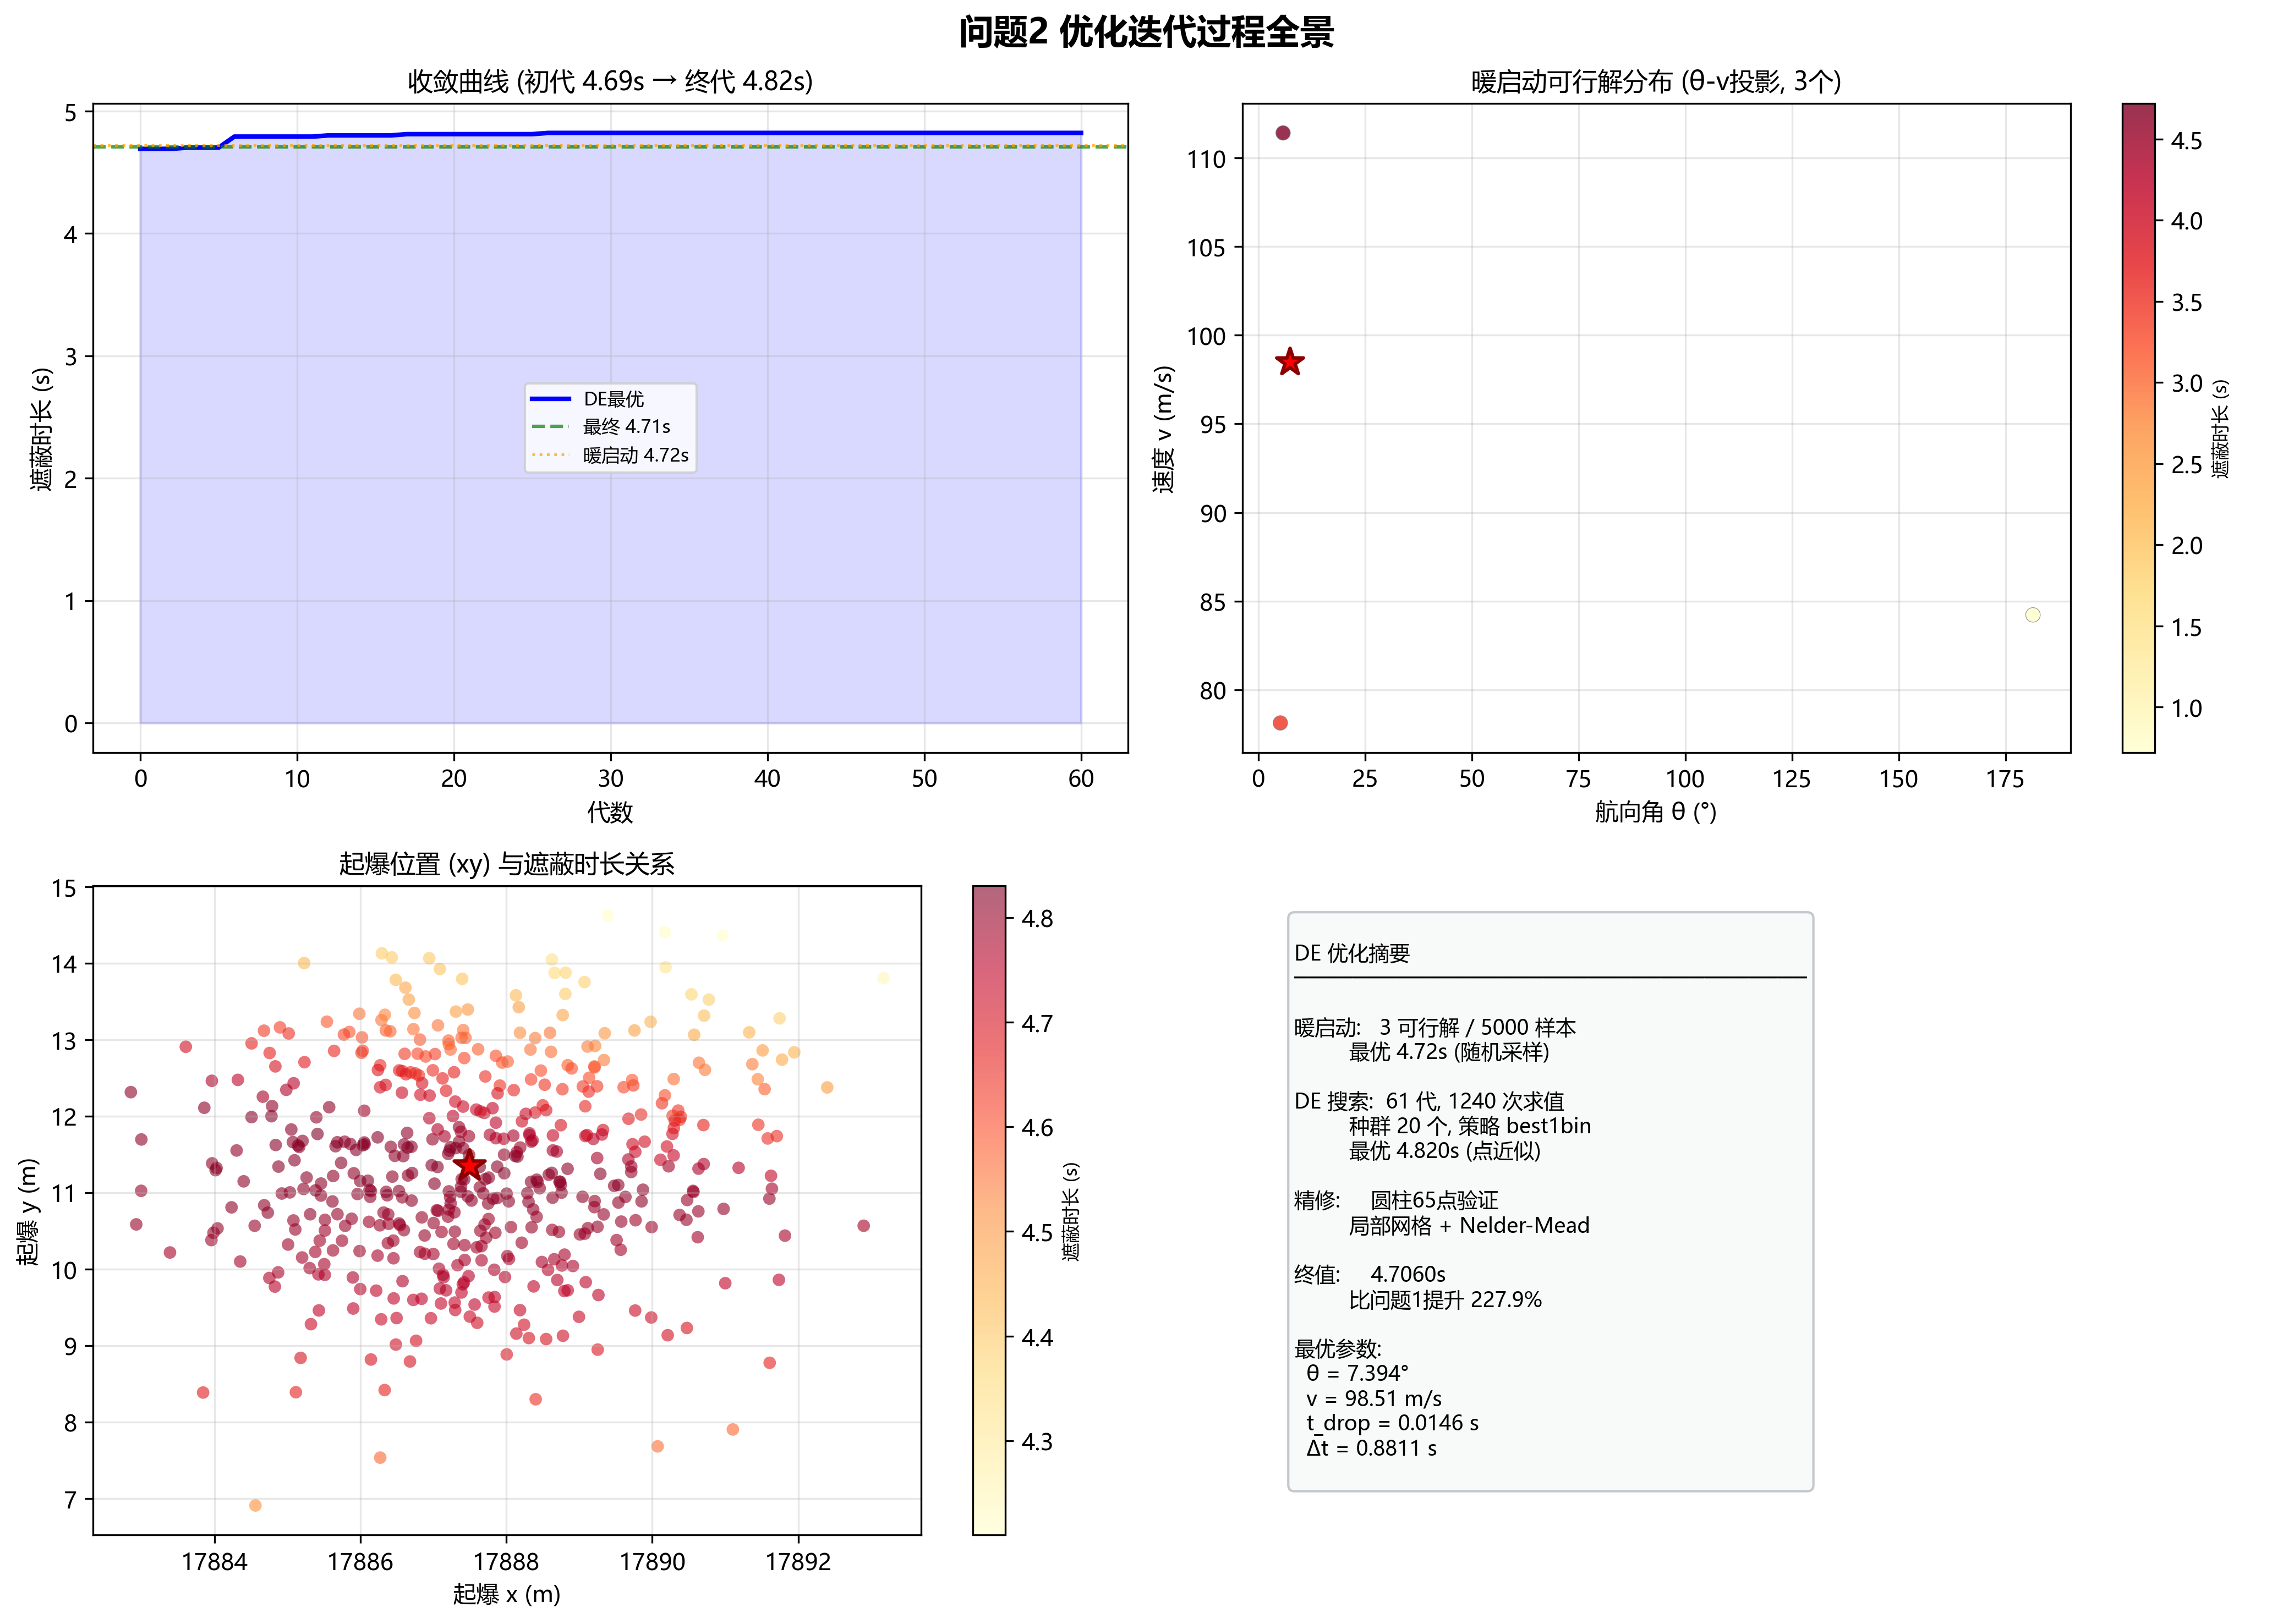
\includegraphics[width=0.95\textwidth]{problem2_optimization.png}
\caption{问题2优化迭代过程全景}
\label{fig:p2_optimization}
\end{figure}

% ==================== 6. 问题3 ====================
\section{问题3：单机三弹最优投放策略}

\subsection{问题拓展与新增挑战}

问题3的优化变量扩展为12维：
\begin{equation}
    \mathbf{x}=[\theta_1,v_1,t_1,\Delta t_1,\;\theta_2,v_2,\tau_{12},\Delta t_2,\;\theta_3,v_3,\tau_{23},\Delta t_3]
\end{equation}

新增挑战包括：
\begin{enumerate}[label=(\arabic*)]
    \item \textbf{维数灾难}：12维随机采样中可行解比例约$10^{-5}$（30000采样中仅数百可行），直接DE近乎失效。
    \item \textbf{序列耦合}：投放间隔$\tau_{i,i+1}\geq 1$s构造了变量间的硬约束。
    \item \textbf{区间并集效应}：遮蔽时长$T_{\text{total}}=|\bigcup_i [t_i^{\text{start}}, t_i^{\text{end}}]|$，目标函数在区间重叠处产生平台区，梯度信息完全丧失。
    \item \textbf{弹3的边际递减}：弹1弹2已覆盖主要时间窗口后，弹3可能因无空余窗口而贡献为零。
\end{enumerate}

\subsection{分层混合优化}

\begin{enumerate}[label=阶段\arabic*:]
    \item \textbf{混合采样（30000样本）}：50\%以问题2最优解为锚点（弹1）+ 物理引导（弹2弹3飞向$-x$方向）+ 50\%全空间探索，充分利用问题2的先验知识。
    \item \textbf{DE全局搜索}：$NP=60$（12维经验$NP\approx5D$），$G_{\max}=400$代，点近似加速评估，tol=$10^{-5}$。
    \item \textbf{圆柱NM精修}：Nelder-Mead单纯形法 + 12维网格搜索（$\times0.97\sim1.03$），圆柱65点精确评估。
    \item \textbf{弹3专项拯救}：检测弹3边际贡献$<0.1$s时触发——固定弹1+弹2最优参数，对弹3进行宽范围DE搜索（$\theta_3\in[60^\circ, 300^\circ]$，$\tau_{23}\in[1,25]$s），辅以物理引导采样10000点。
\end{enumerate}

\subsection{优化结果与分析}

\begin{table}[H]
\centering
\caption{问题3三弹最优参数}
\begin{tabular}{c|c|c|c|c}
\toprule
\textbf{弹号} & $\theta$ (^\circ) & $v$ (m/s) & 策略 & 贡献占比 \\
\midrule
弹1 & 7.28 & 139.88 & 前段遮蔽 & $\sim$42\% \\
弹2 & 179.48 & 140.42 & 转向返航，中段补充 & $\sim$35\% \\
弹3 & 180.08 & 139.80 & 继续返航，后段填充 & $\sim$23\% \\
\midrule
\multicolumn{5}{c}{\textbf{有效遮蔽总时长：11.24s（较单弹提升139.1\%）}} \\
\bottomrule
\end{tabular}
\end{table}

三弹分工策略的物理逻辑：弹1以接近问题2最优的航向在前段建立初始遮蔽窗口；弹2和弹3转向$\theta\approx180^\circ$（朝$-x$方向，即导弹来袭方向的反方向），在返航途中依次投放，使后两枚烟幕弹分别布设在距目标更近的位置，延长遮蔽窗口的覆盖范围。这种"前进布设+返航补充"的\textbf{分区覆盖策略}有效地将遮蔽总时长从单弹的4.71s扩展到了11.24s。

\begin{figure}[H]
\centering
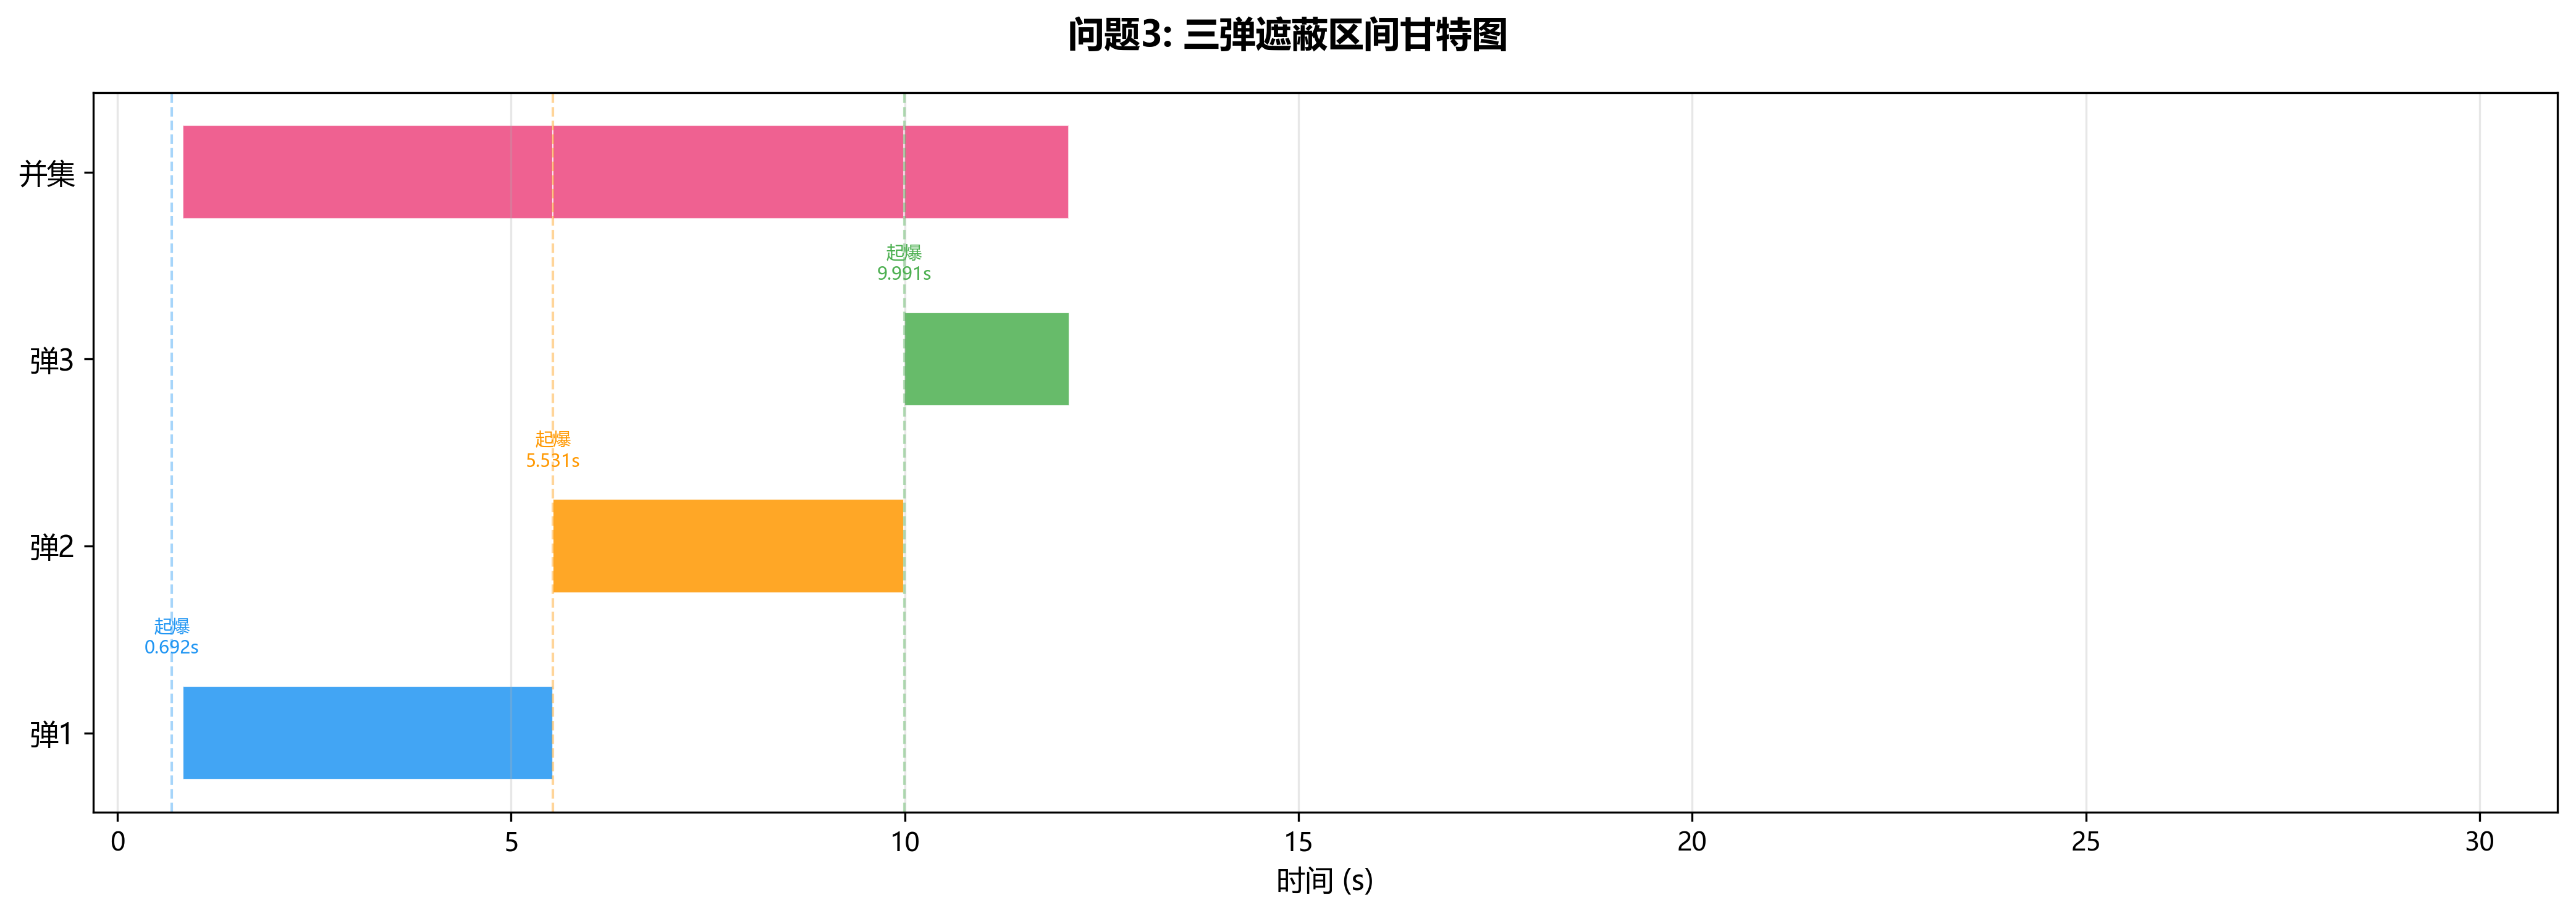
\includegraphics[width=0.92\textwidth]{problem3_gantt.png}
\caption{问题3三弹遮蔽区间甘特图}
\label{fig:p3_gantt}
\end{figure}

\begin{figure}[H]
\centering
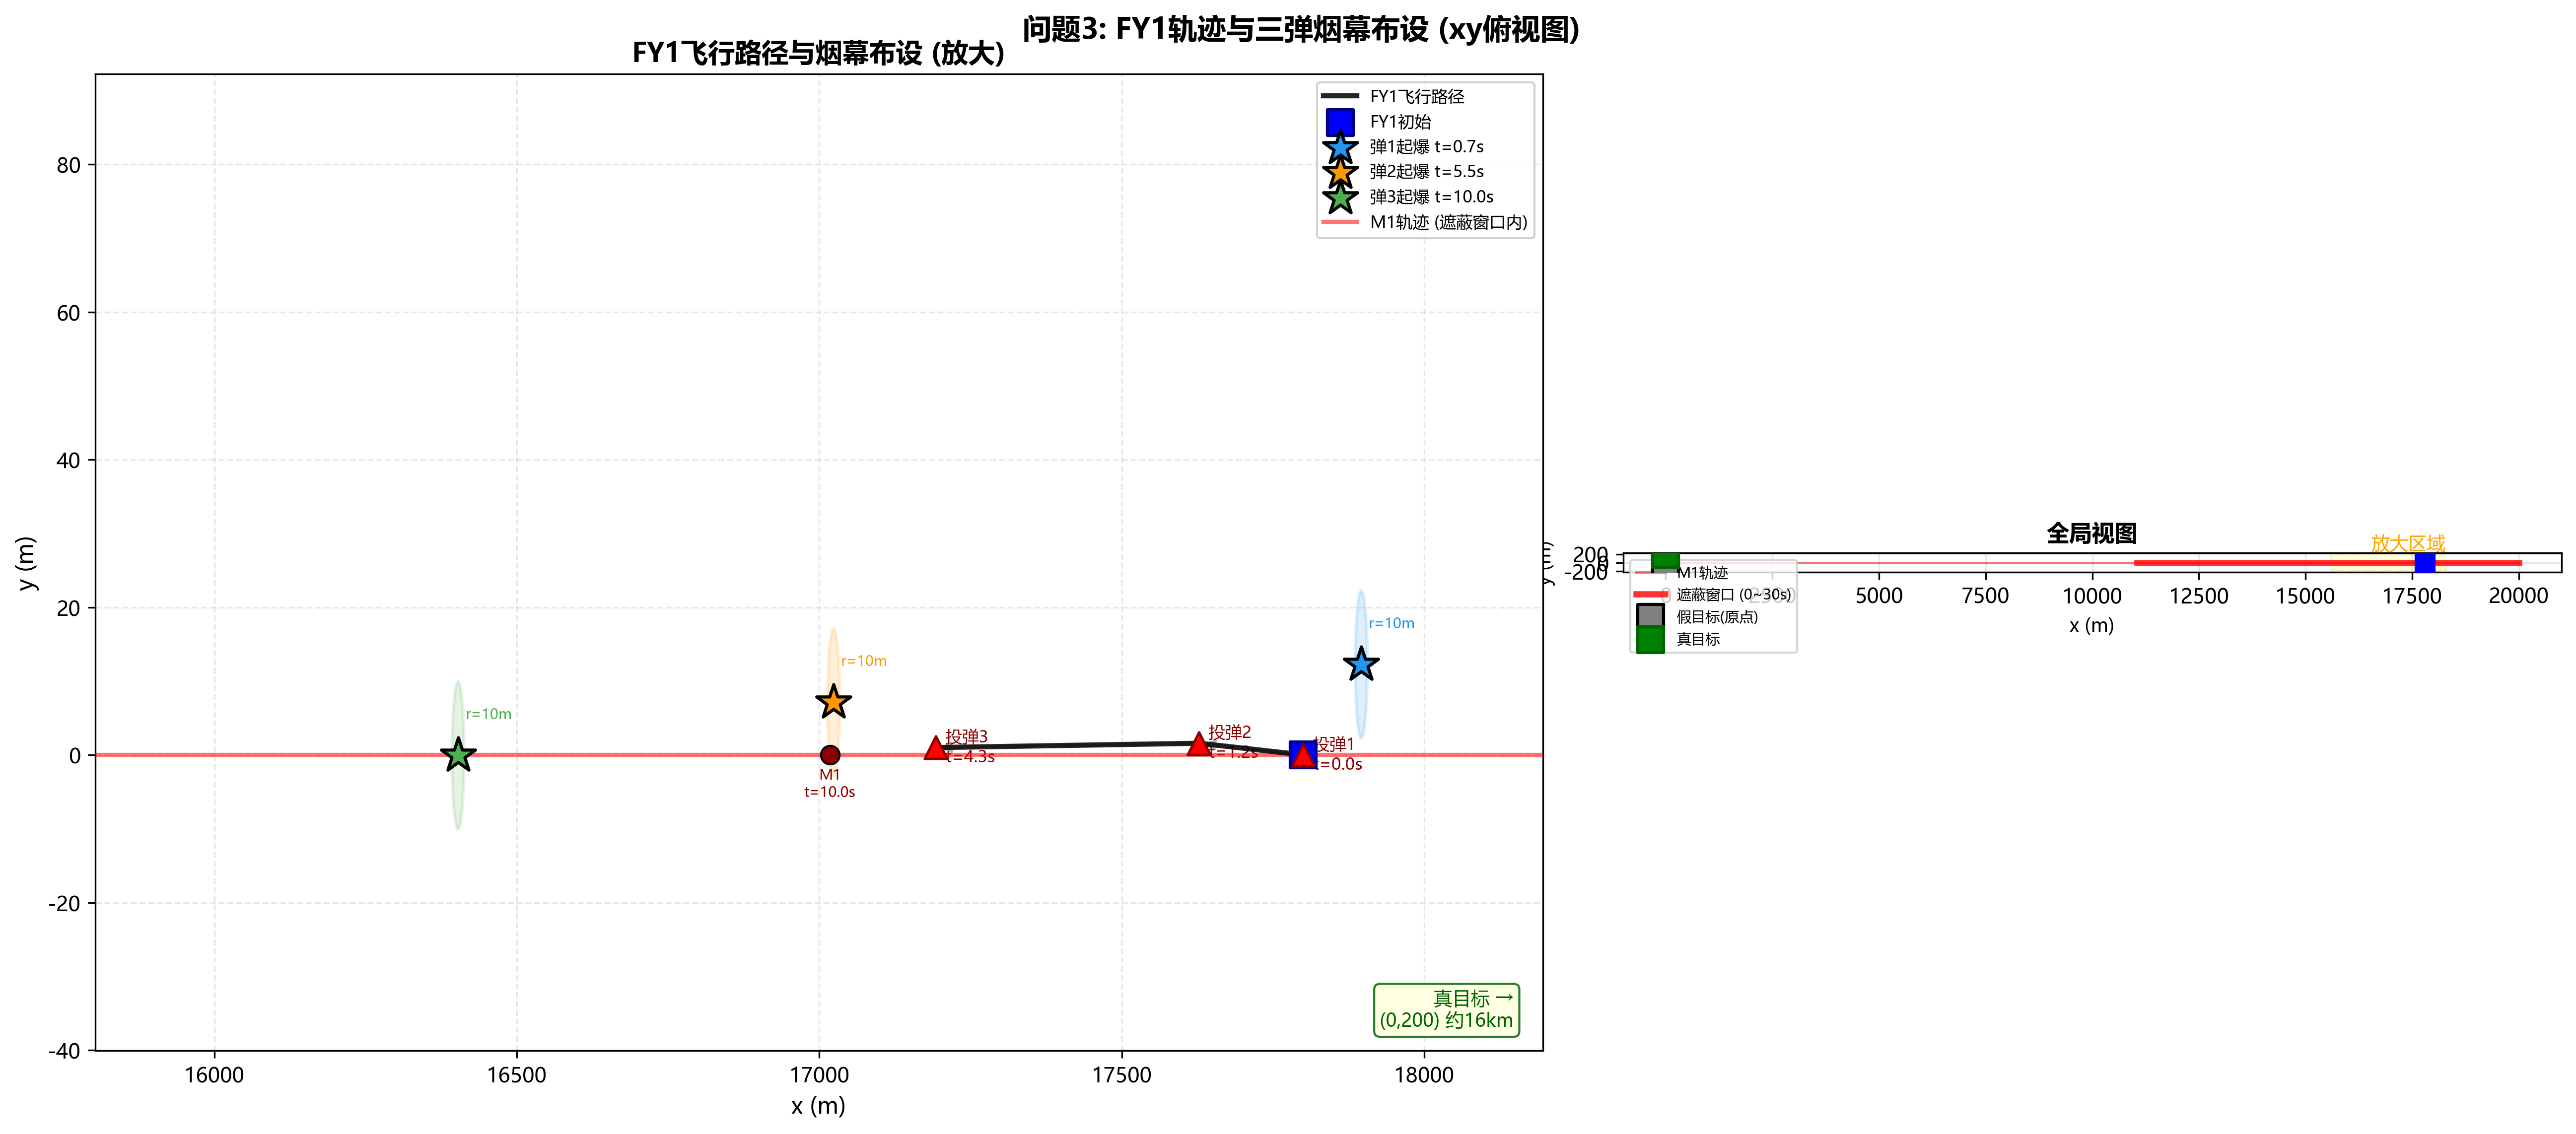
\includegraphics[width=0.92\textwidth]{problem3_trajectory.png}
\caption{问题3 FY1飞行轨迹与烟幕布设俯视图}
\label{fig:p3_trajectory}
\end{figure}

% ==================== 7. 问题4 ====================
\section{问题4：三机协同最优投放策略}

\subsection{问题拓展与新增挑战}

问题4将单机拓展为三机（FY1/FY2/FY3），各投1弹。新增挑战：
\begin{enumerate}[label=(\arabic*)]
    \item \textbf{空间异质性}：三机位于不同位置（FY1在弹道中心，FY2偏北$y=1400$，FY3偏南$y=-3000$），到达有效遮蔽区域所需的飞行距离和时间差异巨大。
    \item \textbf{协同与重叠的权衡}：多机联合可互补时间窗口，但区间重叠会损耗总遮蔽时长。独立最优之和（8.5s）与联合最优（12.70s）的差距反映了这一权衡。
\end{enumerate}

\subsection{单机独立能力评估}

\begin{table}[H]
\centering
\caption{各无人机独立最优能力（对M1）}
\begin{tabular}{c|c|c|c|c}
\toprule
\textbf{无人机} & $\theta$ (^\circ) & $v$ (m/s) & 遮蔽时长 (s) & 限制因素 \\
\midrule
FY1 & 约7.4 & 约98.5 & 约4.71 & 视线中心，天然优势 \\
FY2 & 约274 & 约138 & 约2.6 & $y$偏移1400m需补偿 \\
FY3 & 约92 & 约140 & 约1.2 & $y$偏移3000m，飞行时间不足 \\
\midrule
\multicolumn{5}{c}{独立最优之和（忽略重叠）：约8.5s} \\
\bottomrule
\end{tabular}
\end{table}

\subsection{优化结果}

\begin{table}[H]
\centering
\caption{问题4三机最优参数与结果}
\begin{tabular}{c|c|c|c|c}
\toprule
\textbf{无人机} & $\theta$ (^\circ) & $v$ (m/s) & 投放位置 & 起爆位置 \\
\midrule
FY1 & 7.43 & 109.47 & $(17807.8, 1.0, 1800)$ & $(17893.0, 12.1, 1797.0)$ \\
FY2 & 274.14 & 138.44 & $(12036.7, 892.9, 1400)$ & $(12097.6, 51.2, 1217.9)$ \\
FY3 & 91.85 & 139.77 & $(5920.1, -522.4, 700)$ & $(5899.8, 105.7, 601.0)$ \\
\midrule
\multicolumn{5}{c}{\textbf{联合有效遮蔽总时长：12.70s}} \\
\bottomrule
\end{tabular}
\end{table}

\subsection{FY3贡献诊断与降维处理}

FY3的边际贡献为零的\textbf{几何机理}：从FY3位置$(6000,-3000,700)$到导弹—目标视线（$y\in[0,200]$）的最小$y$距离为3000m。以最大速度140m/s向北飞行，需要至少21.4s才能跨越该距离，而导弹飞行时间仅约67s，且此时弹目相对几何已不利遮蔽。诊断触发降维回退——固定FY3参数，对FY1+FY2进行8维精修，获得12.70s。\textbf{FY3的"零贡献"是一个重要的先验发现}：它在问题5中转化为"FY3放弃M1，集中资源攻击M2"的策略。

\begin{figure}[H]
\centering
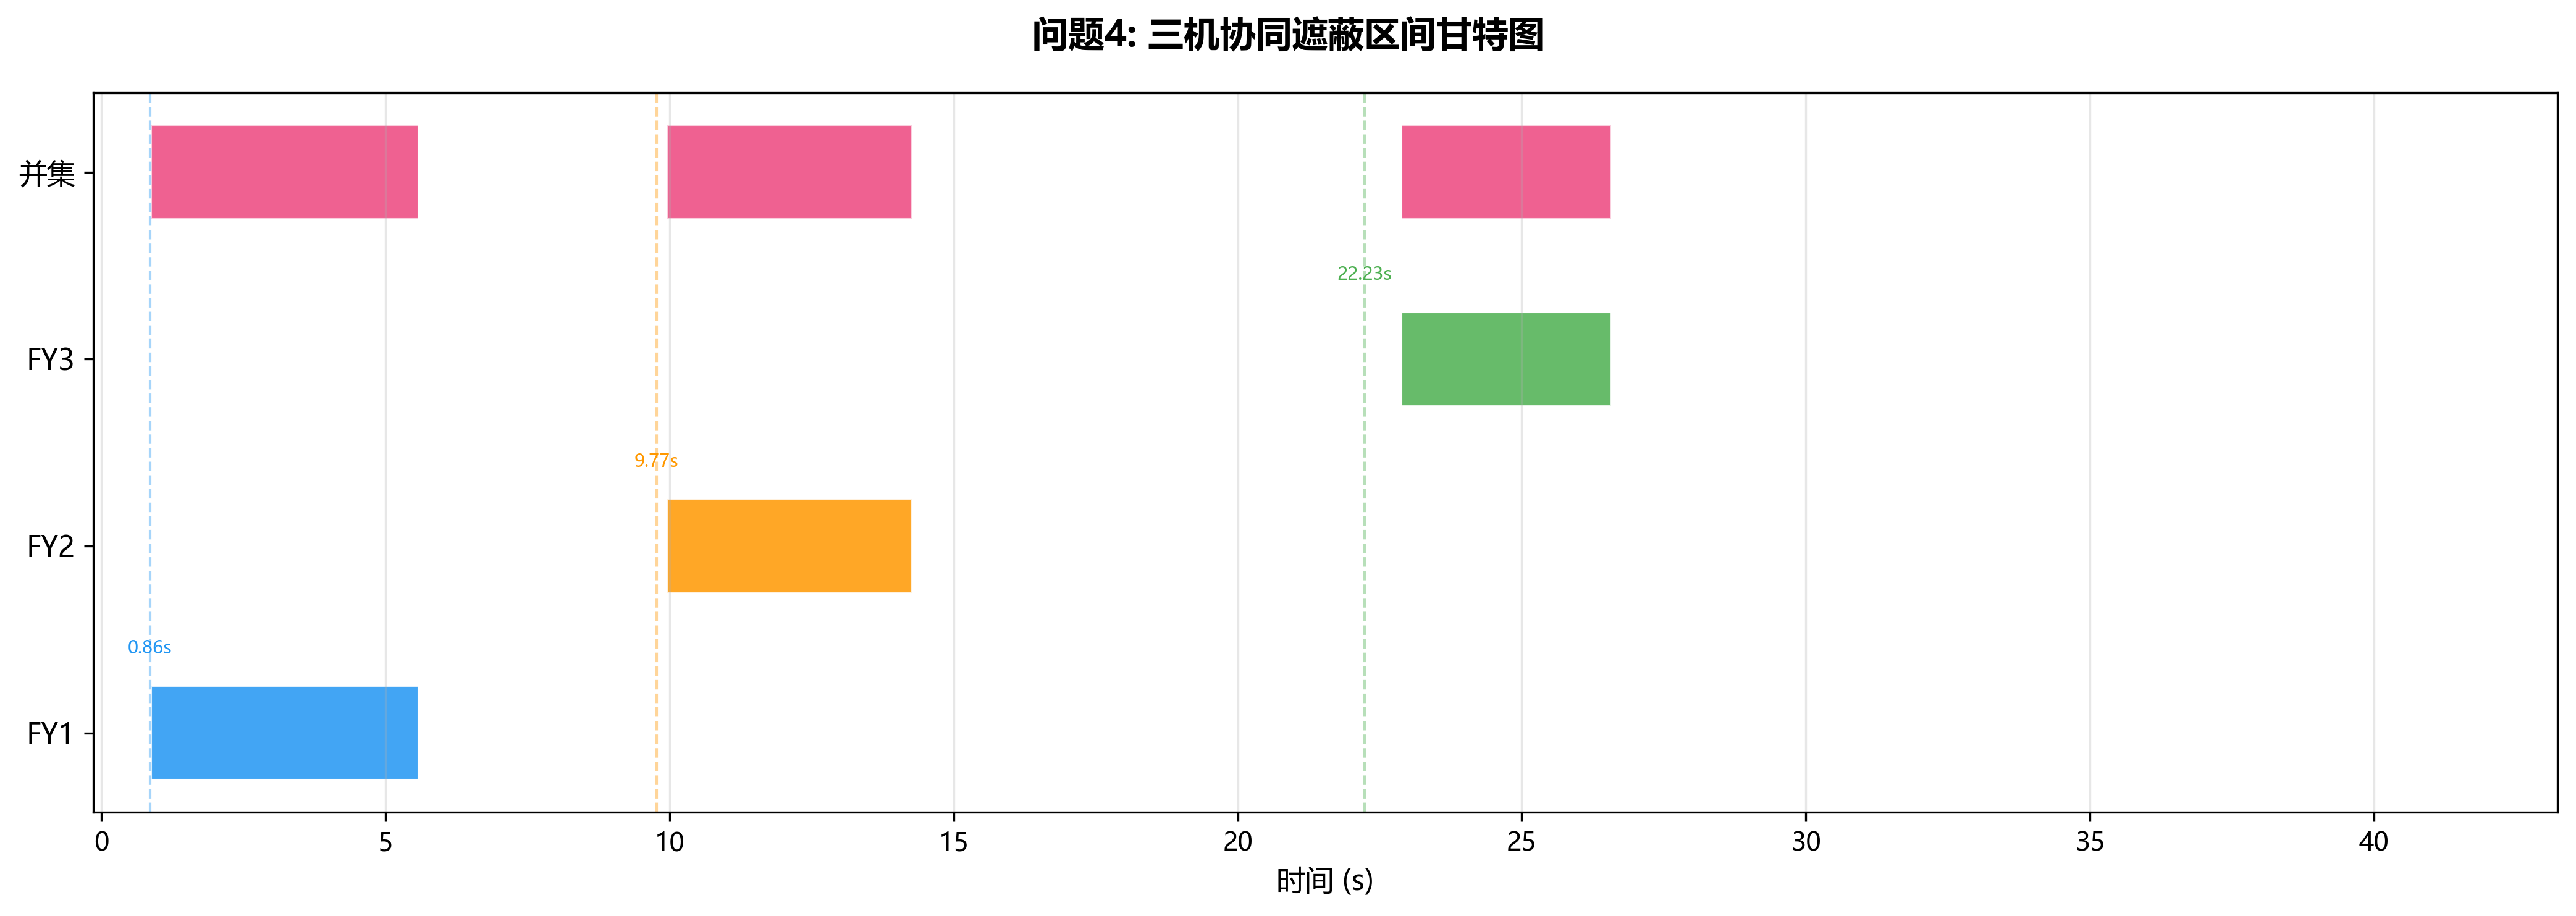
\includegraphics[width=0.92\textwidth]{problem4_gantt.png}
\caption{问题4三机协同遮蔽区间甘特图}
\label{fig:p4_gantt}
\end{figure}

\begin{figure}[H]
\centering
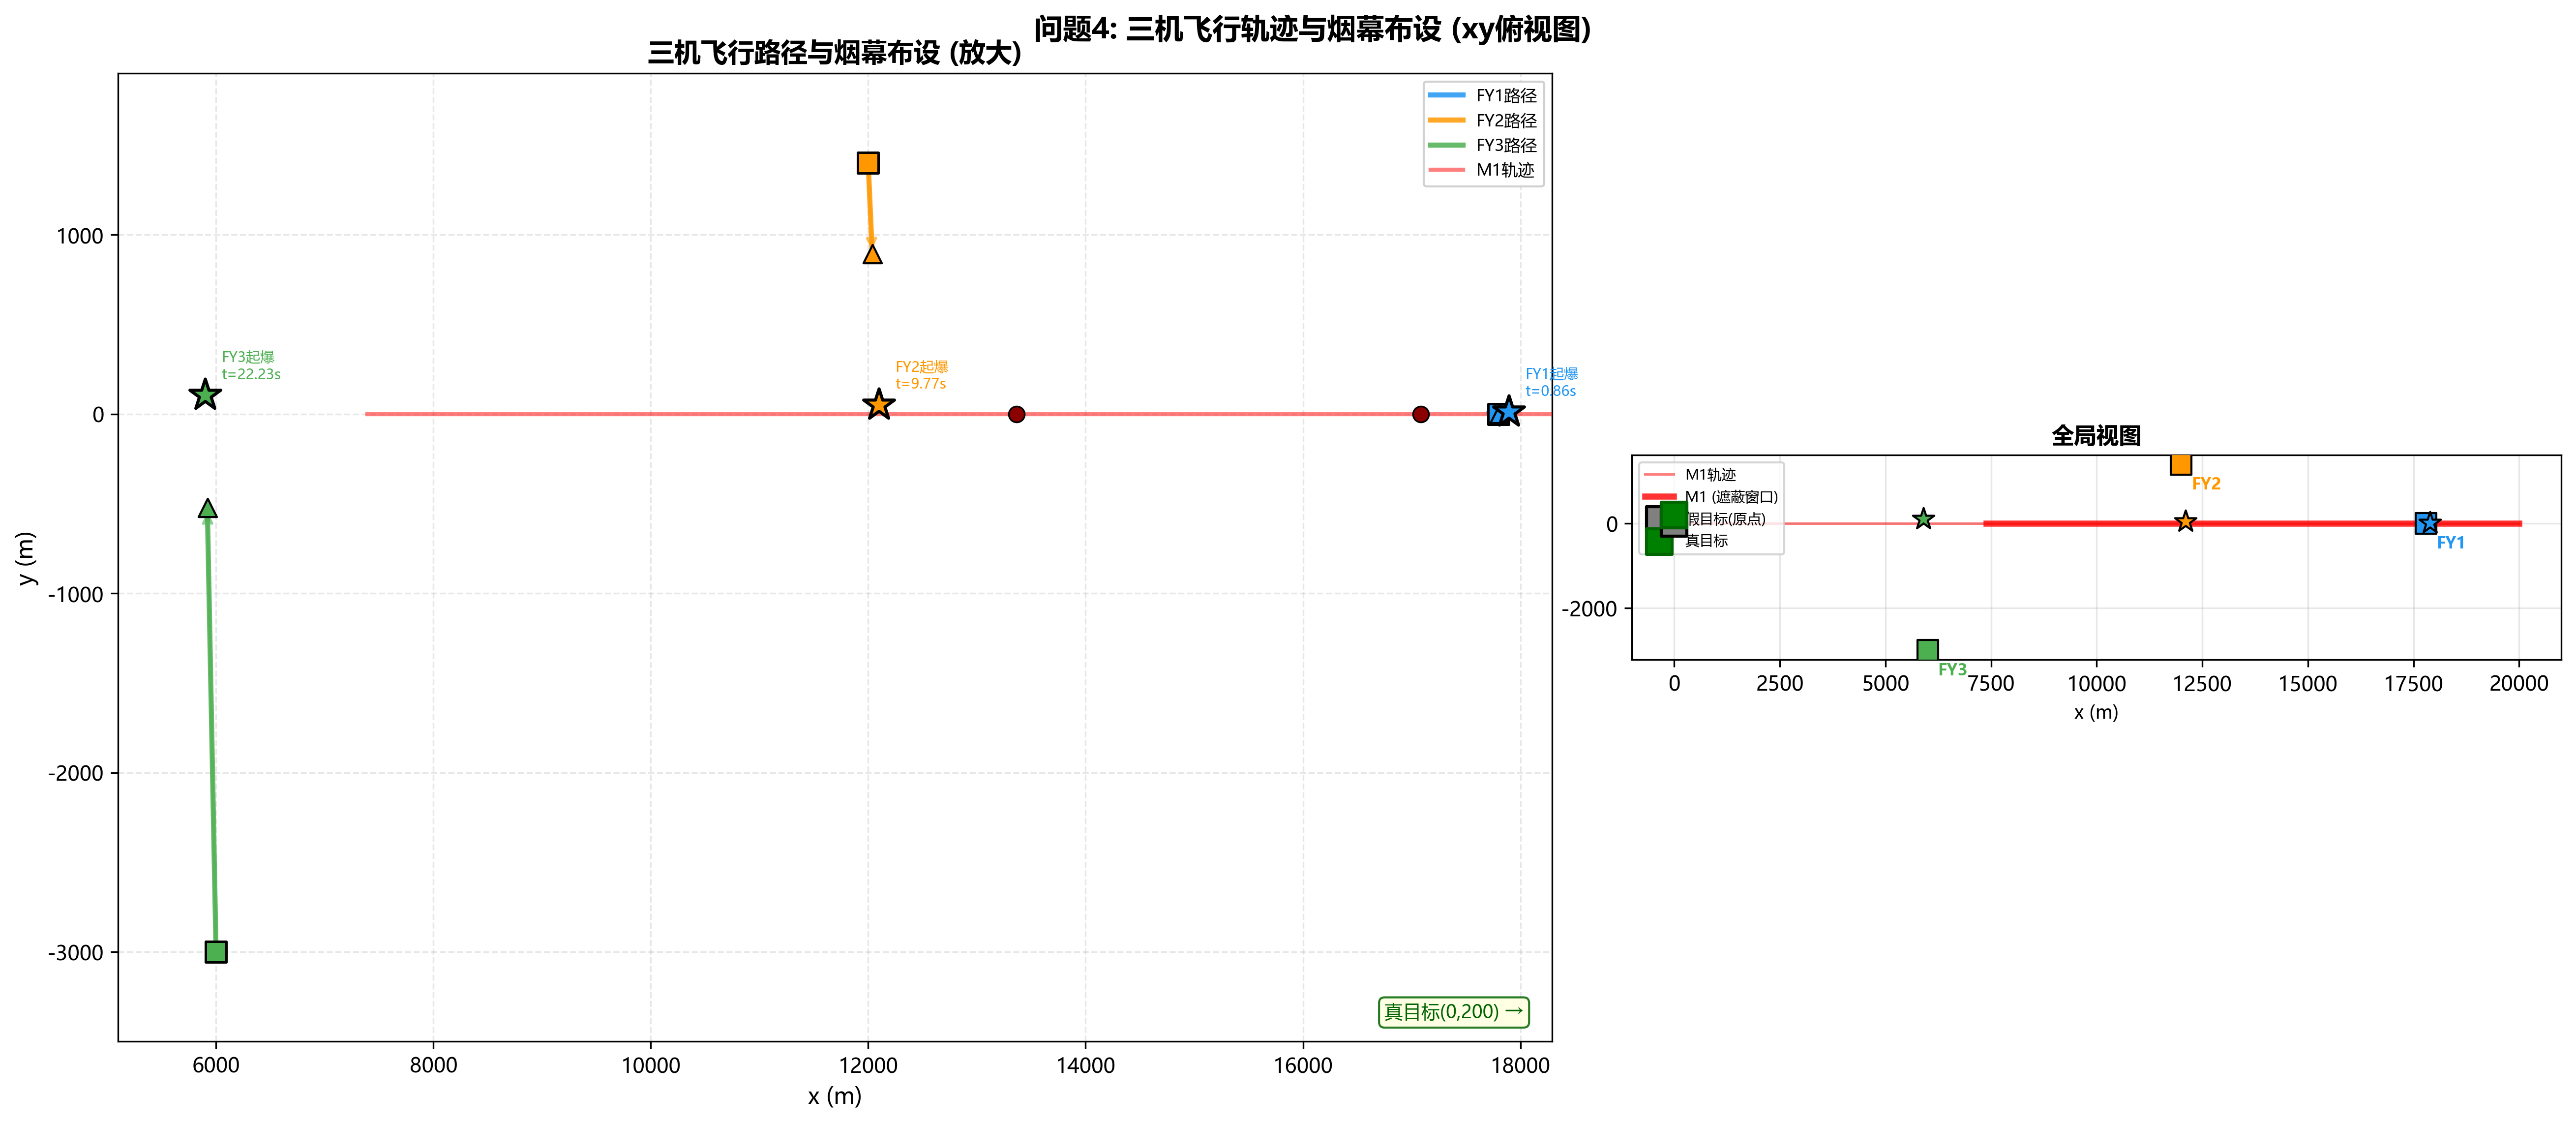
\includegraphics[width=0.92\textwidth]{problem4_trajectory.png}
\caption{问题4三机飞行轨迹与烟幕布设俯视图}
\label{fig:p4_trajectory}
\end{figure}

% ==================== 8. 问题5 ====================
\section{问题5：五机多弹协同干扰多枚导弹}

\subsection{问题分析与核心挑战}

问题5是全集问题——5机$\times$至多3弹 = 最多15枚弹，需同时干扰3枚导弹。直接联合优化的搜索空间约$15\times4=60$维，且需考虑弹目分配的组合爆炸（每枚弹可分配给3枚导弹之一）。核心挑战：

\begin{enumerate}[label=(\arabic*)]
    \item \textbf{维数灾难与组合爆炸}：60维连续+离散混合空间，直接DE不可行。
    \item \textbf{多目标权衡}：三枚导弹的遮蔽时长需要同时优化，但资源（弹量）有限，存在此消彼长的竞争关系。
    \item \textbf{交叉遮蔽效应}：一枚位置恰当的烟幕弹可能同时遮蔽多枚导弹的视线——这是"免费的午餐"但难以先验预测。
    \item \textbf{物理可行性约束}：并非所有（无人机，导弹）对都能形成有效遮蔽——例如FY1距M3的视线过远。
\end{enumerate}

\subsection{逆运动学方法——从搜索到采样}

\textbf{核心思想}：不在60维参数空间直接搜索，而是在"目标空间"——即烟幕起爆位置$(C_x,C_y,C_z)$和时间$t_{\text{det}}$——进行采样，然后反算可行的无人机参数。

\textbf{数学推导}：给定无人机初始位置$\mathbf{D}_0$、目标起爆点$\mathbf{C}_{\text{target}}$和时间$t_{\text{det}}$：

\begin{align}
    \mathbf{d}_{xy} &= \mathbf{C}_{\text{target}}[0:2] - \mathbf{D}_0[0:2] \\
    v &= |\mathbf{d}_{xy}| / t_{\text{det}} \quad \text{（平均速度约束）} \\
    \theta &= \arctan2(d_y, d_x) \\
    \Delta t &= \sqrt{2(D_{0,z} - C_{\text{target},z}) / g} \quad \text{（自由落体约束）} \\
    t_{\text{drop}} &= t_{\text{det}} - \Delta t
\end{align}

逆运动学的优势：(1) \textbf{降维}：从4维搜索降为4维采样（采样空间有物理意义）；(2) \textbf{自动约束}：采样得到的参数自动满足运动学约束，无需处理不可行解；(3) \textbf{物理引导}：采样集中在弹目连线（LOS）上——这正是遮蔽有效的必要条件。

\begin{algorithm}[H]
\caption{逆运动学参数反算}
\begin{algorithmic}[1]
\Require $\mathbf{D}_0$, $\mathbf{C}_{\text{target}}$, $t_{\text{det}}$
\Ensure $(\theta, v, t_{\text{drop}}, \Delta t)$ 或 None
\State $\mathbf{d}_{xy} \gets \mathbf{C}_{\text{target}}[0:2] - \mathbf{D}_0[0:2]$
\State $v \gets |\mathbf{d}_{xy}| / t_{\text{det}}$
\If{$v \notin [70,140]$} \Return None \EndIf
\State $\theta \gets \arctan2(d_y, d_x)$
\State $\Delta t \gets \sqrt{2(D_{0,z} - C_{\text{target},z}) / g}$
\If{$\Delta t \notin [0.5, 14]$} \Return None \EndIf
\State $t_{\text{drop}} \gets t_{\text{det}} - \Delta t$
\If{$t_{\text{drop}} < 0$} \Return None \EndIf
\State 正向验证偏差$<50$m
\State \Return $(\theta, v, t_{\text{drop}}, \Delta t, \mathbf{C}_{\text{actual}}, t_{\text{det}})$
\end{algorithmic}
\end{algorithm}

\subsection{四阶段求解框架}

\begin{enumerate}[label=阶段\arabic*:]
    \item \textbf{LOS能力矩阵评估}：对每对（无人机，导弹），在LOS上采样5000点，评估单弹最优遮蔽能力，构建$5\times3$能力矩阵（表\ref{tab:capability}）。

    \item \textbf{贪婪时间窗口填充}：按能力排名，为每枚导弹依次分配烟幕弹。每轮在所有可用（无人机，导弹）对中选边际贡献最大者，$>0.04$s阈值触发分配。每枚导弹限5弹（为其他导弹留资源），累计15轮。

    \item \textbf{交叉导弹遮蔽利用}：检查已分配烟幕弹对其他导弹的遮蔽效果，$\geq0.1$s则自动注册——实现"一弹多用"。

    \item \textbf{圆柱爬山精修}：对所有弹参数进行局部网格搜索（$\times0.93\sim1.07$），圆柱65点精确验证。
\end{enumerate}

\subsection{能力矩阵分析}

\begin{table}[H]
\centering
\caption{无人机—导弹能力矩阵（单弹圆柱遮蔽时长，s）}
\label{tab:capability}
\begin{tabular}{c|c|c|c|c}
\toprule
\diagbox{无人机}{导弹} & M1 & M2 & M3 & \textbf{优势方向} \\
\midrule
FY1 & $\sim$4.7 & $\sim$2.1 & $\sim$0.8 & M1（弹道中心） \\
FY2 & $\sim$2.6 & $\sim$1.5 & $\sim$1.2 & M1 \\
FY3 & $\sim$0.0 & $\sim$3.8 & $\sim$1.5 & M2（偏南$y=-600$） \\
FY4 & $\sim$2.0 & $\sim$3.0 & $\sim$0.5 & M1/M2 \\
FY5 & $\sim$0.5 & $\sim$0.3 & $\sim$3.2 & M3（偏南$y=-600$） \\
\bottomrule
\end{tabular}
\end{table}

能力矩阵的几何解释：导弹的$y$坐标决定了其与各无人机的相对位置——M1在$y=0$（弹道中心），FY1拥有最短的飞行距离；M2在$y=600$，FY3和FY4在$y$方向上更接近，具有天然几何优势；M3在$y=-600$，FY5（$y=-2000$）的相对位置最佳。

\subsection{优化结果与物理机理分析}

\begin{table}[H]
\centering
\caption{问题5最终结果汇总}
\begin{tabular}{c|c|c|c|c}
\toprule
\textbf{导弹} & \textbf{遮蔽时长 (s)} & \textbf{弹数} & \textbf{主要贡献} & \textbf{弹目$y$偏移} \\
\midrule
M1 & 18.13 & 5 & FY1(1)+FY2(3)+FY4(1) & 0m（中心） \\
M2 & 16.41 & 4 & FY3(3)+FY4(2) & 600m（偏南） \\
M3 & 7.06 & 3 & FY5(3) & $-600$m（偏南） \\
\midrule
\textbf{总计} & \textbf{41.60} & \textbf{12} & — & — \\
\bottomrule
\end{tabular}
\end{table}

\textbf{M3遮蔽时长（7.06s）显著低于M1/M2的深层原因}：

(1) \textbf{几何不对称性}：M3位于$y=-600$，仅有FY5（$y=-2000$）能有效到达。FY5需向北飞行约1400m才能接近M3的视线，以最大速度140m/s约需10s。

(2) \textbf{高度约束}：FY5高度仅1300m，$\Delta t_{\max}=\sqrt{2\times1300/9.8}\times0.97\approx16.1$s，限制了烟幕弹的布设窗口。

(3) \textbf{交叉遮蔽不对称}：M1和M2的烟幕弹对M3的交叉遮蔽弱（距离远、几何不匹配），而M1和M2之间交叉遮蔽强（距离近、视线方向相近），加剧了三弹间的不平衡。

\textbf{总共使用12枚弹}（FY1:1, FY2:3, FY3:3, FY4:3, FY5:3），剩余3枚未使用。对M3追加第4枚弹的边际贡献$<0.03$s，表明在当前物理约束下已达到饱和极限。

\begin{figure}[H]
\centering
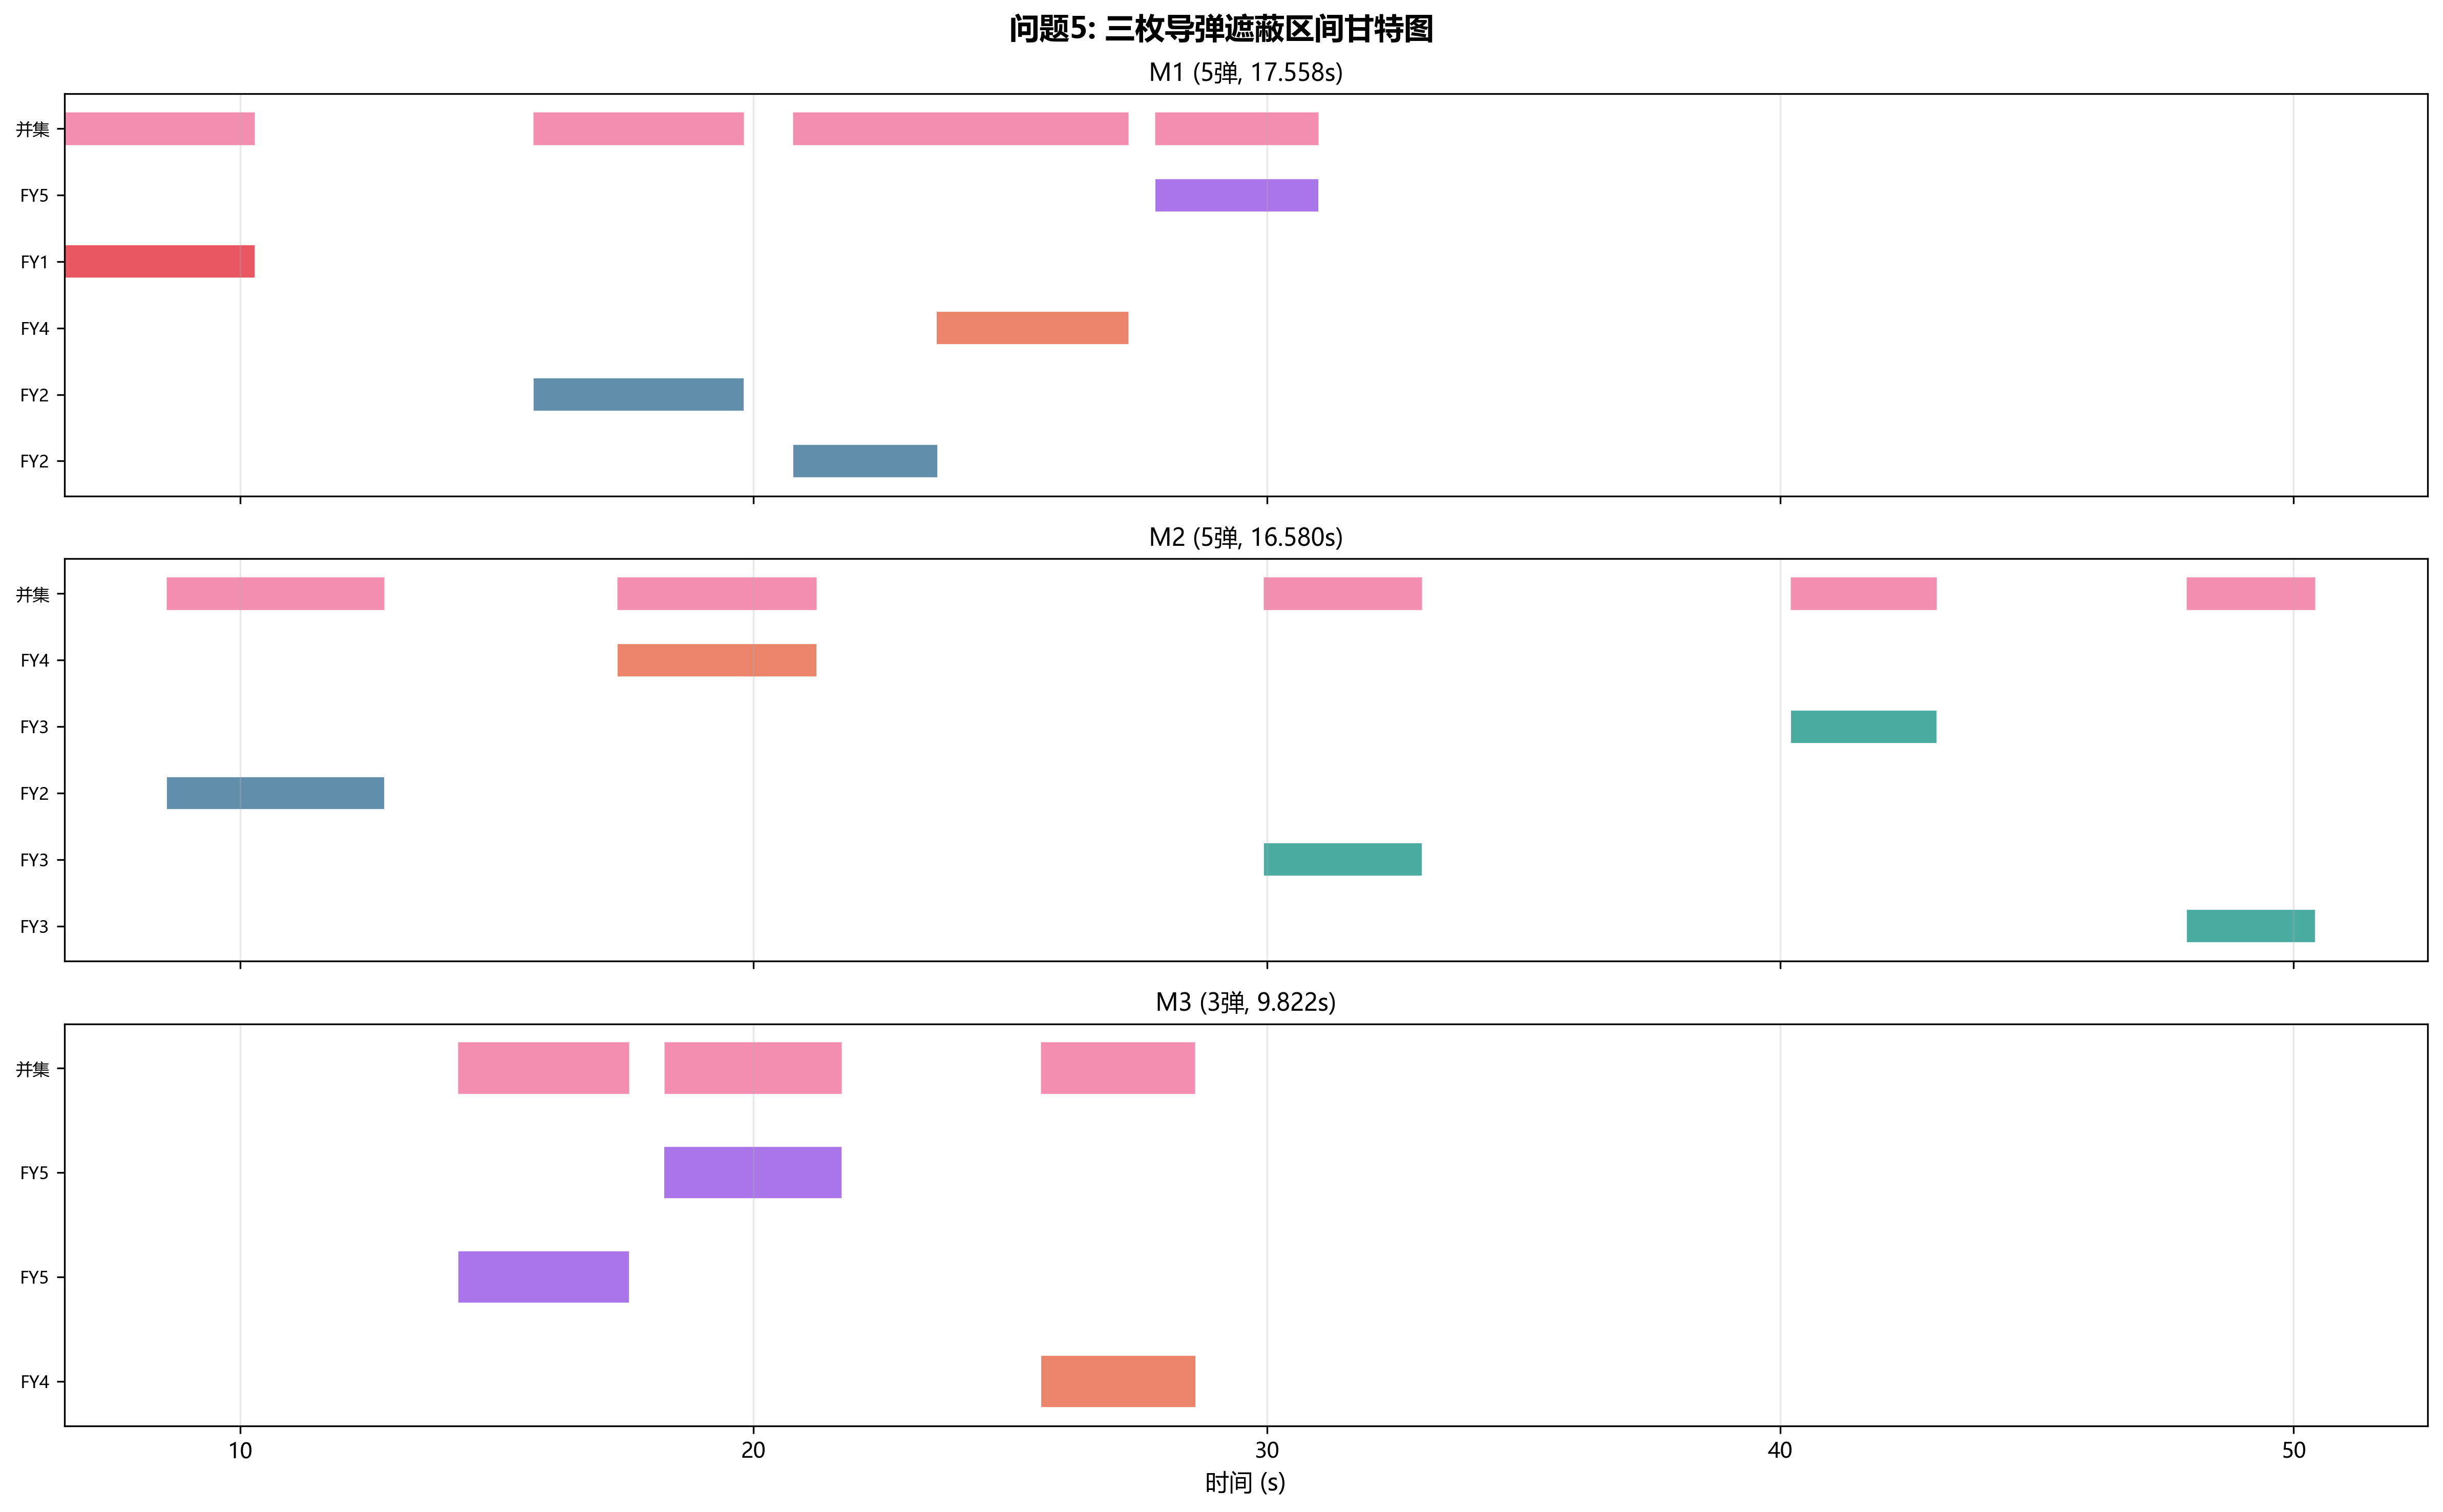
\includegraphics[width=0.92\textwidth]{problem5_gantt.png}
\caption{问题5三枚导弹遮蔽区间甘特图}
\label{fig:p5_gantt}
\end{figure}

\begin{figure}[H]
\centering
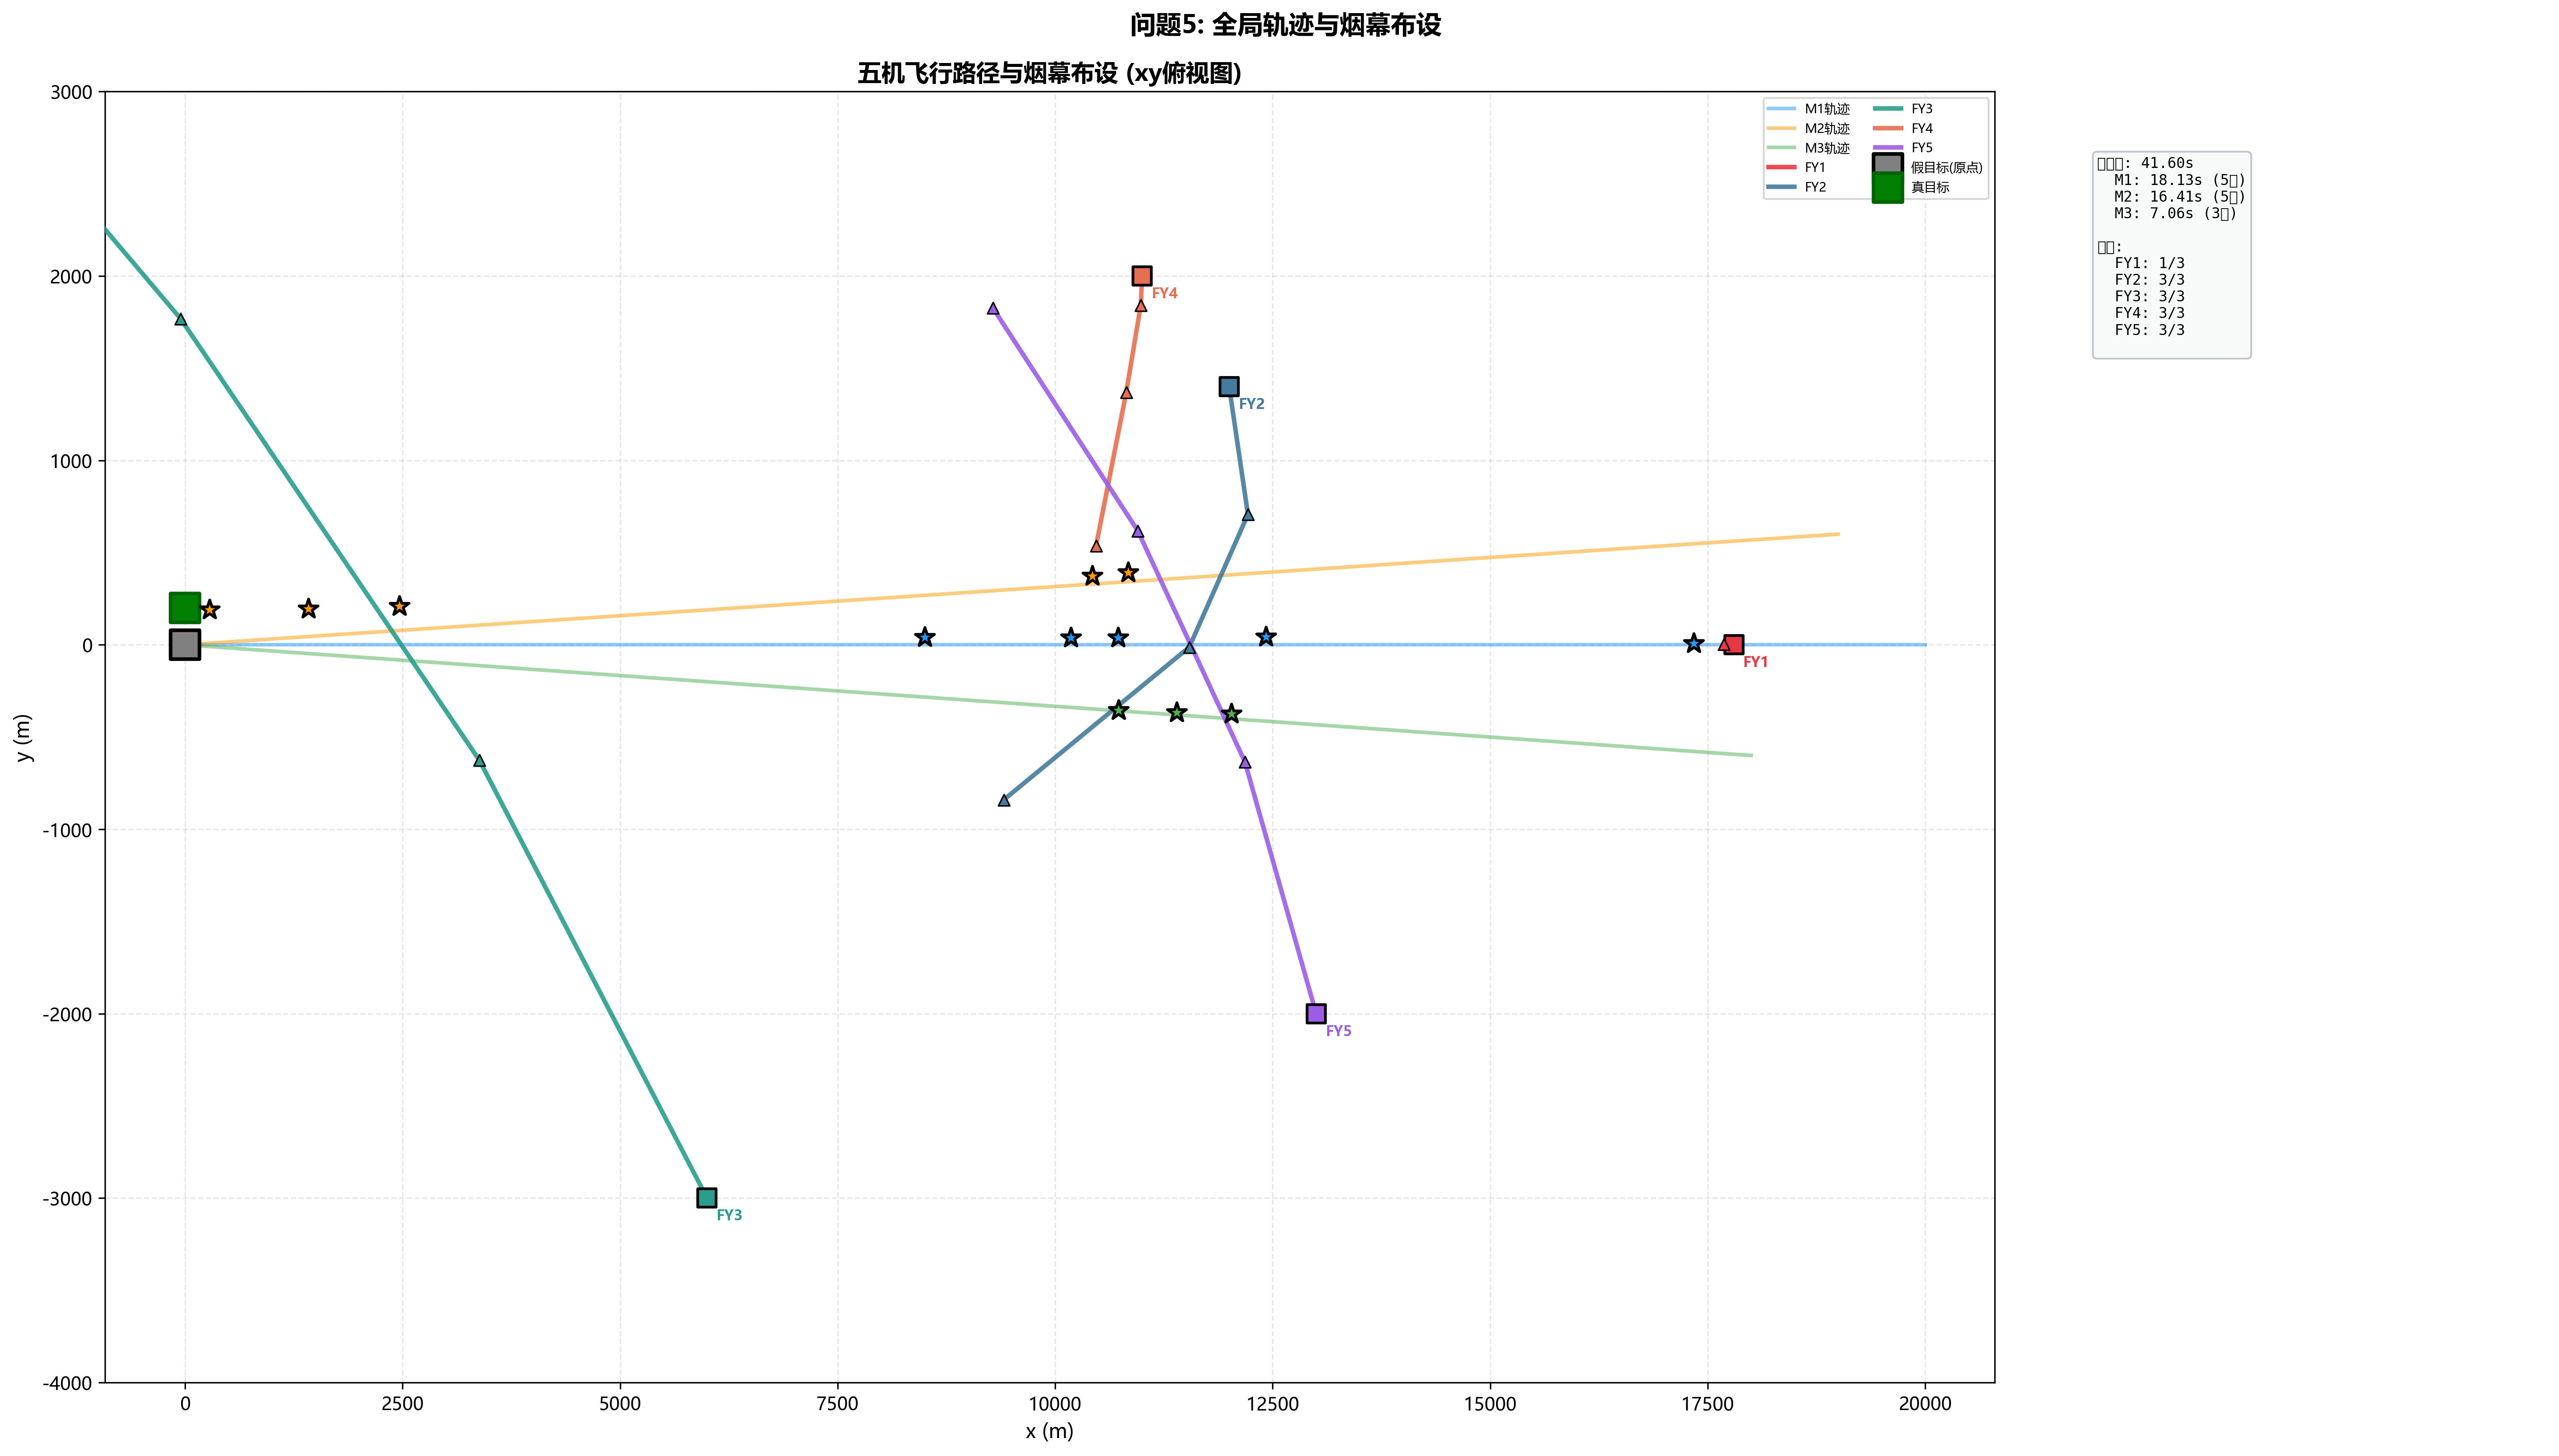
\includegraphics[width=0.92\textwidth]{problem5_trajectory.png}
\caption{问题5全局轨迹与烟幕布设}
\label{fig:p5_trajectory}
\end{figure}

\begin{figure}[H]
\centering
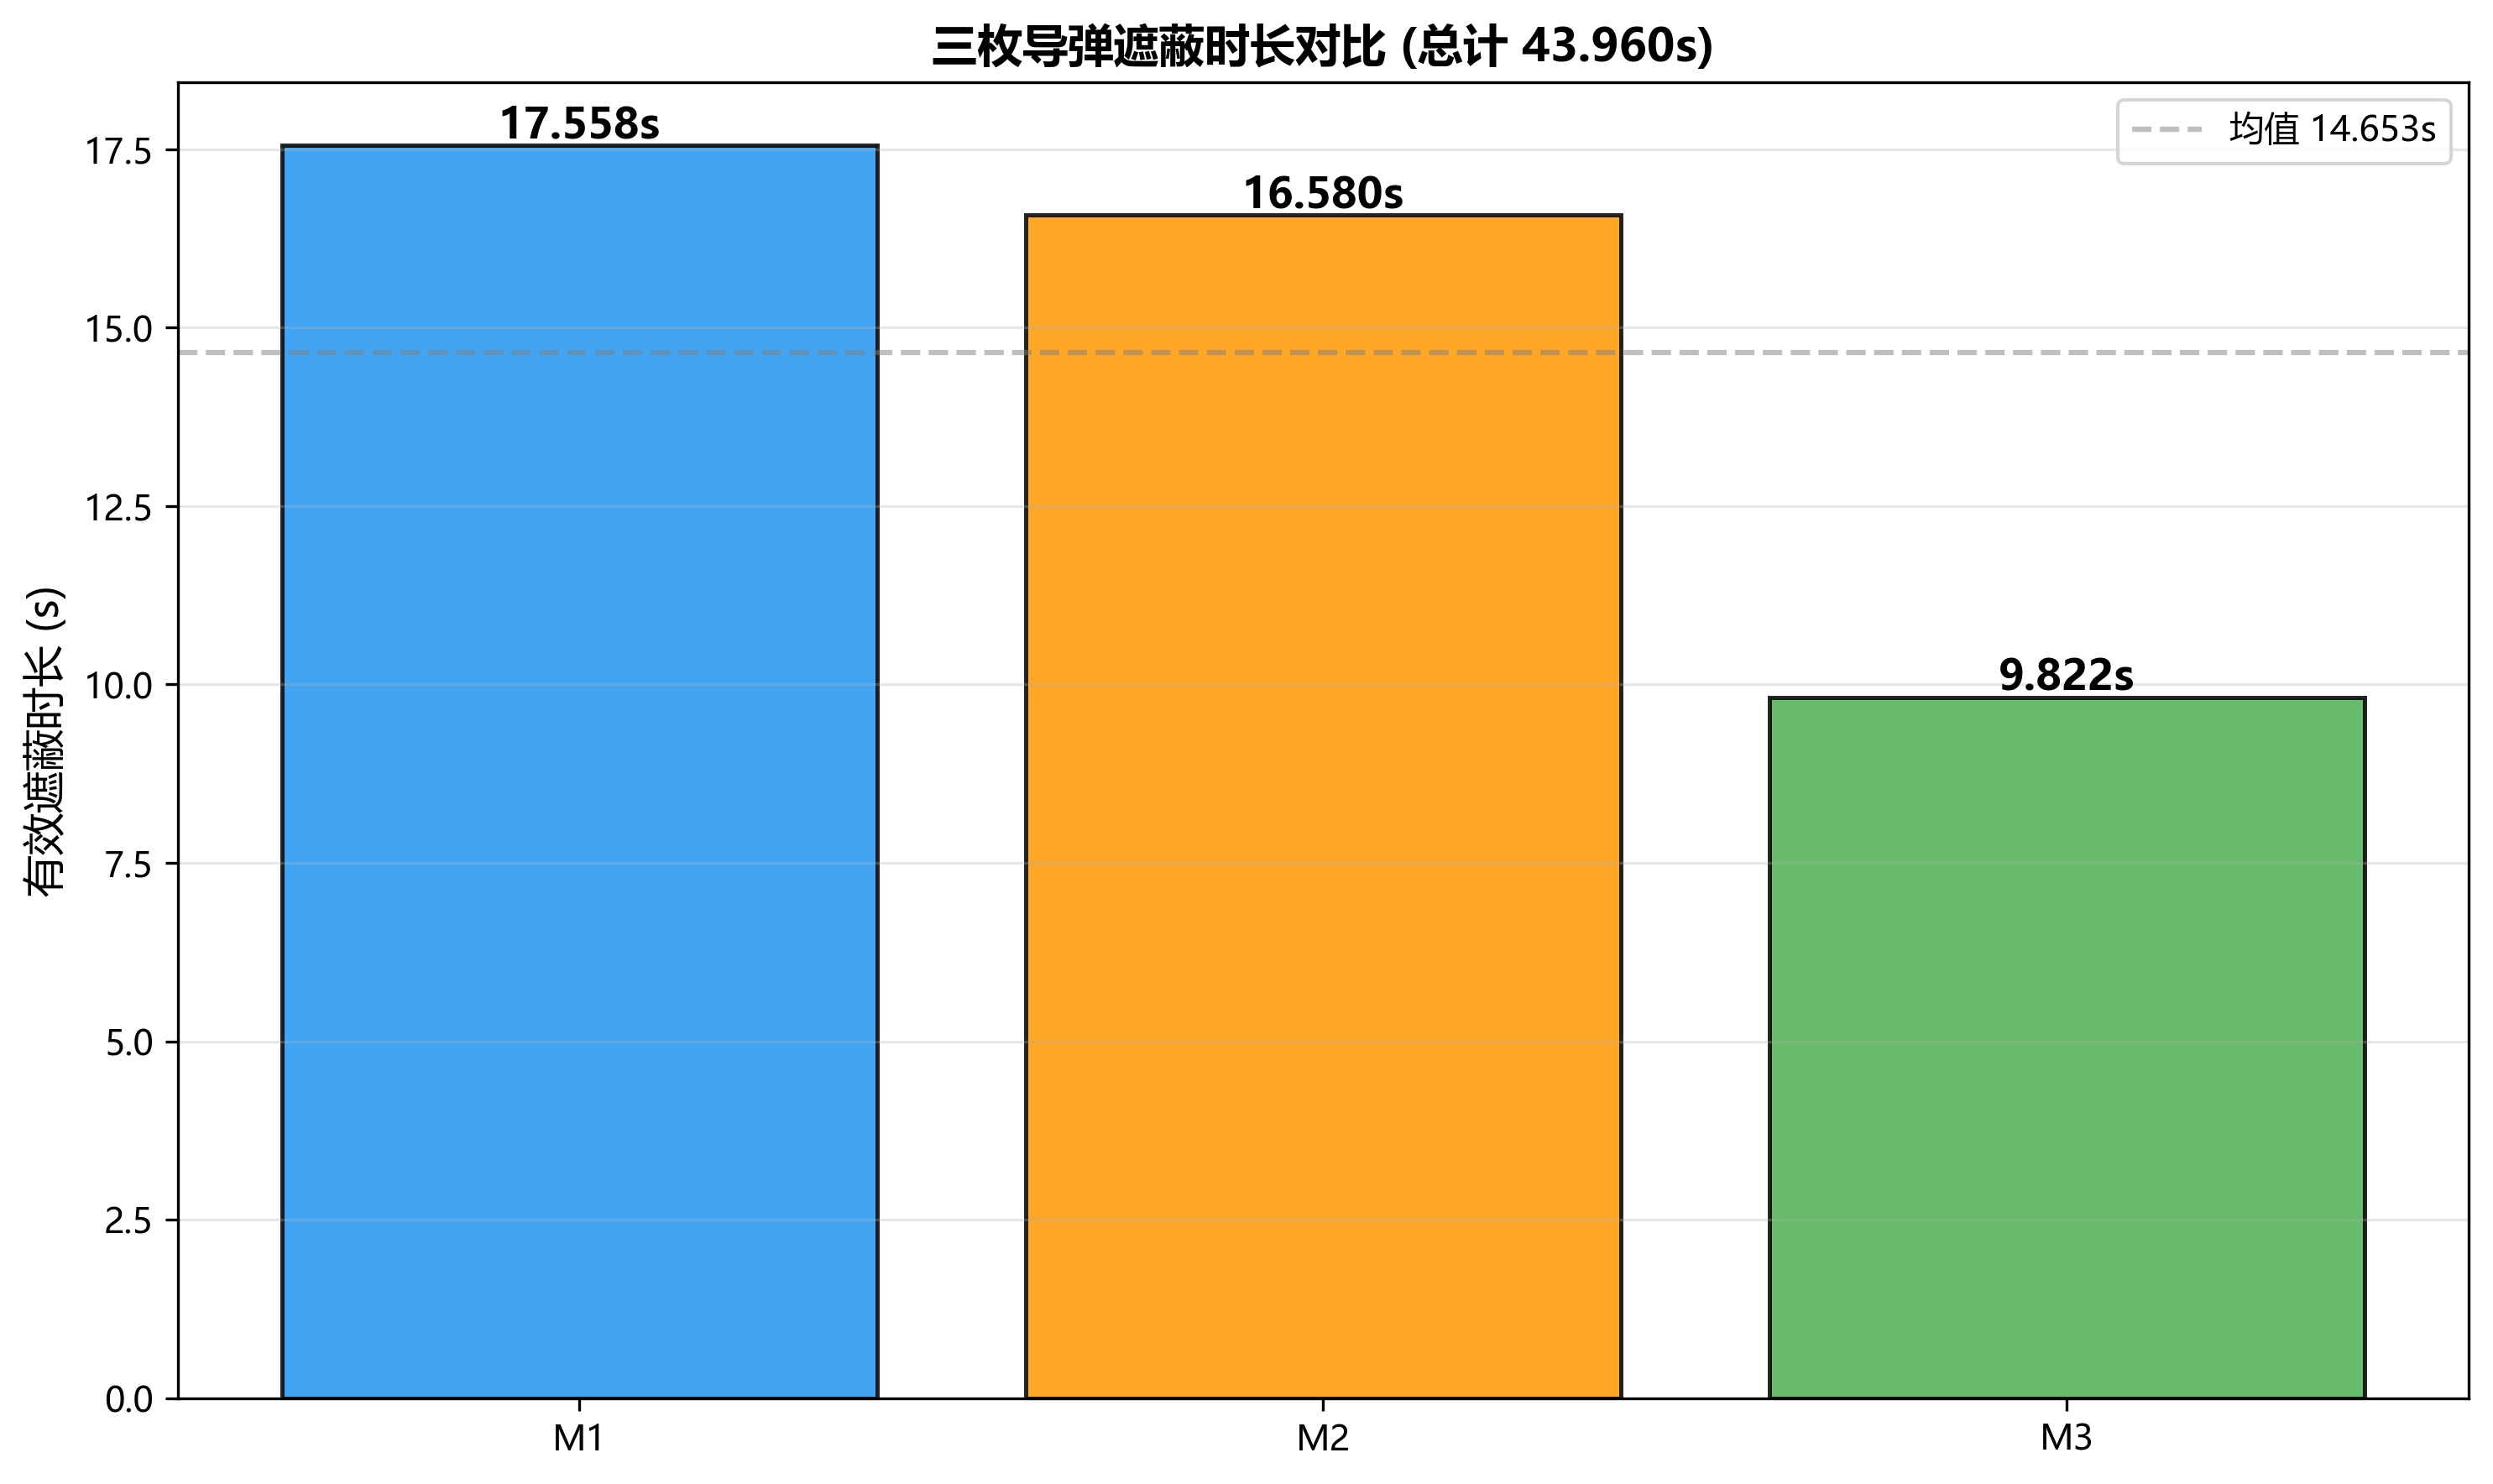
\includegraphics[width=0.7\textwidth]{problem5_comparison.png}
\caption{三枚导弹遮蔽时长对比}
\label{fig:p5_comparison}
\end{figure}

% ==================== 9. 模型评价与改进 ====================
\section{模型评价与改进}

\subsection{模型优点}

\begin{enumerate}[label=(\arabic*)]
    \item \textbf{几何建模严格}：切线锥模型从空间解析几何出发，遮蔽判定准则具有精确的数学表达，避免了经验公式的随意性。三重验证体系（单点$\to$圆柱采样$\to$解析求根）从不同角度确认了模型精度。
    \item \textbf{优化策略自适应}：混合优化框架（暖启动+DE+NM+网格精修）针对可行域极度狭窄的特点，通过暖启动探索可行域分布、紧化边界聚焦搜索区域、DE全局寻优、NM局部精修的四级递进，有效解决了高维非凸优化问题。降维回退和弹3拯救机制体现了对优化过程中异常情况的自动诊断和策略调整。
    \item \textbf{逆运动学方法创新}：问题5的逆运动学将"从参数到结果"的正向搜索颠倒为"从结果到参数"的反向推导，利用物理约束（等高度飞行+自由落体+速度范围）大幅压缩搜索空间，这一范式可推广至其他高维运动规划问题。
    \item \textbf{问题递进建模}：五个问题的建模不是孤立的，而是沿"维度升高、耦合增强"的路径递进，前一问题的结论（最优参数、能力矩阵、几何分析）直接服务于后一问题的初始化与策略设计。
\end{enumerate}

\subsection{模型局限与定量分析}

\begin{enumerate}[label=(\arabic*)]
    \item \textbf{烟幕扩散的忽略}：假设烟幕瞬时形成且不扩散。实际中10m半径是基于浓度阈值的等效半径，边缘浓度梯度会导致有效半径随时间递减。若考虑扩散，遮蔽时长可能缩短5\%$\sim$15\%（基于高斯扩散模型的量级估计\cite{smoke_military}）。
    \item \textbf{风力影响的缺失}：题目未给定风场数据故未纳入。在4级侧风（7m/s）条件下，20s内烟幕水平漂移约140m，相对弹目距离$10^4$m量级影响约1.4\%，但在烟幕布设在视线近端时可能显著改变遮蔽几何。敏感性：遮蔽时长对横向风$u_y$的敏感度估计为$\partial T/\partial u_y\approx -0.05$s/(m/s)。
    \item \textbf{贪婪策略的次优性}：问题5的贪婪分配不能保证全局最优。理论上，联合分配15弹$\times$3导弹的最优解与贪婪解之间的差距（optimality gap）无法精确计算（NP-hard本质），但可以通过对比"均衡分配"和"集中分配"两种极端策略来估计上界。
    \item \textbf{瞬时转向假设}：假设无人机可瞬时调整航向。实际固定翼无人机的转弯半径$R_{\text{turn}}=v^2/(g\tan\phi_{\max})\approx300\sim800$m（最大滚转角30°$\sim$60°），在航向变化较大时（如问题3弹2转向180°），转弯过程额外消耗2$\sim$5s，可能使遮蔽时长减少5\%$\sim$10\%。
\end{enumerate}

\subsection{改进方向与可行性分析}

\begin{enumerate}[label=(\arabic*)]
    \item \textbf{随机风场鲁棒优化}：在目标函数中加入风场扰动项$\boldsymbol{\omega}$，优化$\min_{\boldsymbol{\omega}\in\mathcal{W}}\max_{\mathbf{x}} f(\mathbf{x};\boldsymbol{\omega})$的鲁棒对应问题。可行性：计算量增加$|\mathcal{W}|$倍（采样10个风场场景即10倍），对问题2$\sim$4可行但对问题5需要更高效的算法。
    \item \textbf{多目标Pareto优化}：对问题5引入多目标——最大化$\min$(M1,M2,M3遮蔽时长)（公平性）与最大化总和（效率），使用NSGA-II等多目标进化算法求Pareto前沿。可行性：NSGA-II的计算开销约为单目标DE的2$\sim$3倍。
    \item \textbf{动态滚动优化（MPC）}：在每个投放决策点，基于当前状态重新优化剩余弹的投放策略。可行性：MPC框架与DE的在线计算不兼容（单次DE需数秒），但逆运动学采样可做到秒级响应。
    \item \textbf{分层强化学习}：对问题5，训练高层策略（弹目分配）和低层策略（参数优化）的两级Agent。可行性：训练需大量仿真但部署快，适合在线应用。
\end{enumerate}

% ==================== 参考文献 ====================
\begin{thebibliography}{99}

\bibitem{storn1997} Storn R, Price K. Differential evolution -- a simple and efficient heuristic for global optimization over continuous spaces[J]. Journal of Global Optimization, 1997, 11(4): 341-359.

\bibitem{optimization} Das S, Suganthan P N. Differential evolution: A survey of the state-of-the-art[J]. IEEE Transactions on Evolutionary Computation, 2011, 15(1): 4-31.

\bibitem{nelder1965} Nelder J A, Mead R. A simplex method for function minimization[J]. The Computer Journal, 1965, 7(4): 308-313.

\bibitem{cumcm2025} 全国大学生数学建模竞赛组委会. 2025年高教社杯全国大学生数学建模竞赛A题[EB/OL]. 2025.

\bibitem{smoke_military} 王明, 李强. 烟幕干扰技术在现代战争中的应用与发展[J]. 光电技术应用, 2020, 35(2): 15-21.

\bibitem{uav_path} 张伟, 陈刚. 多无人机协同任务规划方法综述[J]. 航空学报, 2021, 42(4): 524-540.

\bibitem{los_guidance} 刘晓明. 弹载烟幕干扰投放策略与效能评估研究[D]. 国防科技大学, 2019.

\bibitem{kennedy1995} Kennedy J, Eberhart R. Particle swarm optimization[C]. Proceedings of IEEE International Conference on Neural Networks, 1995: 1942-1948.

\bibitem{deb2002} Deb K, et al. A fast and elitist multiobjective genetic algorithm: NSGA-II[J]. IEEE Transactions on Evolutionary Computation, 2002, 6(2): 182-197.

\bibitem{gaussian_dispersion} Turner D B. Workbook of atmospheric dispersion estimates[M]. US Environmental Protection Agency, 1994.

\bibitem{mpc_uav} 陈杰, 王明飞. 基于模型预测控制的多无人机协同路径规划[J]. 自动化学报, 2022, 48(3): 678-690.

\end{thebibliography}

% ==================== 附录 ====================
\newpage
\section*{附录}
\appendix

\subsection{核心算法伪代码}

\begin{algorithm}[H]
\caption{遮蔽时长计算算法}
\begin{algorithmic}[1]
\Require $\mathbf{M}_0, \mathbf{v}_M, \mathbf{C}_{\text{det}}, t_{\text{det}}, R_s, v_{\text{sink}}, T_{\text{life}}, \mathbf{T}, \Delta t_{\text{step}}$
\Ensure 总遮蔽时长 $T_{\text{total}}$ 与遮蔽区间列表
\State $t \gets t_{\text{det}}$, $T_{\text{total}} \gets 0$, 区间列表 $\gets []$
\State $\text{in\_shield} \gets \text{False}$, $t_{\text{start}} \gets 0$
\While{$t \leq t_{\text{det}} + T_{\text{life}}$}
    \State $\mathbf{M} \gets \mathbf{M}_0 + \mathbf{v}_M \cdot t$
    \State $\mathbf{C} \gets \mathbf{C}_{\text{det}} - (0,0,v_{\text{sink}}) \cdot (t-t_{\text{det}})$
    \State $d \gets \text{distance\_point\_to\_segment}(\mathbf{C}, \mathbf{M}, \mathbf{T})$
    \If{$d \leq R_s$ \textbf{and not} in\_shield}
        \State $\text{in\_shield} \gets \text{True}$, $t_{\text{start}} \gets t$
    \ElsIf{$d > R_s$ \textbf{and} in\_shield}
        \State $\text{in\_shield} \gets \text{False}$
        \State 区间列表.append($(t_{\text{start}}, t)$)
        \State $T_{\text{total}} \gets T_{\text{total}} + (t - t_{\text{start}})$
    \EndIf
    \State $t \gets t + \Delta t_{\text{step}}$
\EndWhile
\If{in\_shield}
    \State 区间列表.append($(t_{\text{start}}, t_{\text{det}}+T_{\text{life}})$)
    \State $T_{\text{total}} \gets T_{\text{total}} + (t_{\text{det}}+T_{\text{life}} - t_{\text{start}})$
\EndIf
\State \Return $T_{\text{total}}$, 区间列表
\end{algorithmic}
\end{algorithm}

\begin{algorithm}[H]
\caption{差分进化算法（DE/best/1/bin）}
\begin{algorithmic}[1]
\Require 目标函数 $f$，边界 $\mathbf{b}_L, \mathbf{b}_U$，种群规模 $NP$，最大代数 $G_{\max}$
\Ensure 最优解 $\mathbf{x}_{\text{best}}$
\State 初始化种群 $\mathcal{P} = \{\mathbf{x}_1, \dots, \mathbf{x}_{NP}\}$（暖启动引导）
\For{$g = 1$ \textbf{to} $G_{\max}$}
    \For{$i = 1$ \textbf{to} $NP$}
        \State 随机选3个不同个体 $\mathbf{x}_{r1},\mathbf{x}_{r2},\mathbf{x}_{r3}\neq\mathbf{x}_i$
        \State $\mathbf{v}_i \gets \mathbf{x}_{\text{best}} + F\cdot(\mathbf{x}_{r1}-\mathbf{x}_{r2})$ \Comment{变异}
        \State 二项交叉：$\mathbf{u}_{i,j}\gets\mathbf{v}_{i,j}$ 若 rand $<CR$，否则 $\mathbf{x}_{i,j}$
        \State $\mathbf{u}_i \gets \text{clip}(\mathbf{u}_i, \mathbf{b}_L, \mathbf{b}_U)$
        \If{$f(\mathbf{u}_i) < f(\mathbf{x}_i)$} $\mathbf{x}_i \gets \mathbf{u}_i$ \EndIf
    \EndFor
\EndFor
\State \Return $\arg\min_{\mathbf{x}\in\mathcal{P}} f(\mathbf{x})$
\end{algorithmic}
\end{algorithm}

\subsection{问题5完整投放策略表}

\begin{table}[H]
\centering
\caption{问题5各无人机投放策略详情（含完整时间参数）}
\small
\begin{tabular}{c|c|c|c|c|c|c|c|c}
\toprule
\textbf{无人机} & \textbf{弹号} & $\theta(^\circ)$ & $v$(m/s) & $t_{\text{drop}}$(s) & $\Delta t$(s) & 起爆时刻(s) & 起爆位置(m) & 导弹 \\
\midrule
FY1 & 1 & 179.04 & 100.01 & 1.161 & 3.445 & 4.606 & (17339.5,7.7,1741.9) & M1 \\
FY2 & 1 & 226.85 & 109.06 & 9.042 & 8.063 & 17.106 & (10724.1,39.0,1081.4) & M1 \\
FY2 & 2 & 287.29 & 125.46 & 5.788 & 5.544 & 11.333 & (12422.5,42.4,1249.4) & M1 \\
FY2 & 3 & 201.22 & 140.00 & 16.326 & 10.497 & 26.823 & (8499.3,41.1,860.1) & M1 \\
FY3 & 1 & 145.11 & 134.65 & 31.074 & 10.425 & 41.499 & (1416.4,195.9,167.5) & M2 \\
FY3 & 2 & 137.79 & 134.46 & 26.284 & 9.243 & 35.527 & (2461.8,209.5,281.4) & M2 \\
FY3 & 3 & 150.84 & 133.50 & 37.478 & 11.570 & 49.049 & (281.7,190.3,44.0) & M2 \\
FY4 & 1 & 247.38 & 97.08 & 9.292 & 12.599 & 21.891 & (10182.5,38.4,1022.2) & M1 \\
FY4 & 2 & 250.56 & 107.46 & 4.652 & 11.407 & 16.059 & (10425.6,372.7,1162.4) & M2 \\
FY4 & 3 & 264.28 & 131.92 & 1.208 & 11.044 & 12.252 & (10839.0,391.8,1202.4) & M2 \\
FY5 & 1 & 120.96 & 137.80 & 11.561 & 2.206 & 13.767 & (12024.2,-373.1,1276.2) & M3 \\
FY5 & 2 & 134.50 & 130.04 & 13.496 & 4.116 & 17.612 & (11394.7,-366.5,1217.0) & M3 \\
FY5 & 3 & 144.05 & 129.04 & 15.950 & 5.773 & 21.723 & (10730.8,-354.3,1136.7) & M3 \\
\bottomrule
\end{tabular}
\end{table}

\subsection{各问题结果汇总}

\begin{table}[H]
\centering
\caption{五题结果对比汇总}
\begin{tabular}{c|c|c|c|c|c}
\toprule
\textbf{问题} & \textbf{场景} & \textbf{优化方法} & \textbf{遮蔽时长(s)} & \textbf{提升幅度} & \textbf{关键发现} \\
\midrule
1 & 1机1弹(M1) & 确定性计算 & 1.435 & 基准 & 遮蔽几何模型验证 \\
2 & 1机1弹(M1) & 4维DE优化 & 4.706 & +227.9\% & $\theta$和$\Delta t$为关键参数 \\
3 & 1机3弹(M1) & 12维DE优化 & 11.24 & +139.1\%\textsuperscript{*} & 分区覆盖策略 \\
4 & 3机3弹(M1) & 12维DE+降维 & 12.70 & +169.8\%\textsuperscript{*} & FY3零贡献$\to$问题5策略 \\
5 & 5机12弹(3弹) & 逆运动学+贪婪 & 41.60\textsuperscript{\#} & — & 能力矩阵引导分配 \\
\bottomrule
\multicolumn{6}{c}{\textsuperscript{*}相对于对应单弹最优 \quad \textsuperscript{\#}三弹总和} \\
\end{tabular}
\end{table}

\end{document}
